\documentclass[journal]{IEEEtran}

\usepackage{graphicx}
\usepackage{booktabs}
\usepackage{array}
\usepackage{cite}
\usepackage{url}
\usepackage[hidelinks]{hyperref}

\graphicspath{{../figures/pdf/}}
\hyphenation{DATATRAIN-CENTER UCIe side-band}

\begin{document}

\title{A Specification-Traceable RTL and Verification Framework for a UCIe 2.0 Link-Training Control Subset}

\author{Author Name(s) to Be Supplied Before Submission%
\thanks{Author names, affiliations, e-mail addresses, ORCIDs, and biographies
must be completed and approved before submission. This pre-submission draft is
not anonymous because IEEE TVLSI is not a blind-submission venue.}}

\markboth{Pre-Submission Technical Draft---September 2026}%
{Author(s): UCIe 2.0-Derived Link-Training Control Subset}

\maketitle

\begin{abstract}
This work presents a specification-traceable register-transfer-level and verification framework for a bounded Universal Chiplet Interconnect Express 2.0-derived link-training control problem. The synthesizable design combines a nine-state hierarchical controller, bounded sideband retry and response matching, a 16-lane 23-bit linear-feedback shift-register measurement engine, retained training-error classification, and a compact field-programmable gate array control/status-register wrapper. Production verification disables the abstract training bypass and independently predicts message order, accepted-sample lane state, strict error-threshold decisions, abort cause, and state advancement. Five fixed seeds execute 180 trials covering nine nominal, retry, malformed-response, pattern-failure, reset, fatal, and timeout classes; accepted logs contain no verification errors or fatals, and 398 independent predictor checks complete. On a Cyclone 10 LP device, the wide diagnostic top fails to fit at the 151-pin package limit, whereas the byte-register wrapper fits with 824 logic elements, 505 registers, and 119 pins. Internal 80-MHz timing reports positive setup and hold slack. The evidence supports a reproducible academic digital-control case study, not a complete physical layer, electrical link, interoperability result, or standards-compliance claim.
\end{abstract}

\begin{IEEEkeywords}
chiplets, FPGA, link training, UCIe, UVM.
\end{IEEEkeywords}

\section{Introduction}
\label{sec:introduction}

Chiplet-based systems partition functions across dies and reconnect them within
a package. This decomposition can improve reuse and allow each function to use
an appropriate process, but it moves system correctness into the die-to-die
interface and package boundary \cite{li2020chiplet,lau2021chiplets}. UCIe
defines an open layered interface intended to support such heterogeneous
integration \cite{sharma2022ucie}. Within its physical-layer control, the Link
Training State Machine (LTSM) coordinates reset, sideband initialization,
mainband initialization and training, active operation, retraining, error, and
low-power behavior \cite{ucie20}.

An academic RTL model of this control is easy to overstate. Listing standard
states does not implement their physical procedures; a passing nominal
simulation does not test message ordering under backpressure; and an FPGA
synthesis report does not establish a working UCIe link. Reproducible negative
evidence is equally important: failed fits, malformed responses, pattern
failure, abort timing, and retained error behavior define the boundary of what
has actually been shown.

This paper presents a source-available, specification-traceable RTL and
verification framework for a UCIe 2.0-derived digital-control subset. The
synthesizable design combines a nine-state hierarchical controller, a bounded
retrying sideband sequencer, a 16-lane 23-bit LFSR measurement engine, retained
TRAINERROR classification, and a compact FPGA CSR wrapper. Its detailed case
study is the production DATATRAINCENTER1 path, in which START completion admits
pattern measurement, pattern failure retries without END, and a matching END
response gates advancement.

The paper makes three bounded contributions:

\begin{enumerate}
\item a modular controller architecture that integrates sideband transaction,
accepted-sample LFSR measurement, error retention, and compact observability
without presenting the result as a complete UCIe PHY;
\item an interface-derived UVM predictor and SVA layer that independently check
message order, per-lane LFSR state, strict threshold semantics, abort cause, and
state advancement; and
\item a reproducible evidence chain comprising directed suites, preserved
multi-seed campaigns, 180 production integrated trials across nine scenario
classes, and qualified Quartus results that retain both a failed wide-top fit
and a successful 119-pin CSR-wrapper fit.
\end{enumerate}

Section~\ref{sec:architecture} defines the implementation boundary and RTL.
Section~\ref{sec:verification} describes prediction, assertions, and scenario
accounting. Section~\ref{sec:evaluation} reports simulation and FPGA evidence.
Sections~\ref{sec:related} and \ref{sec:discussion} position the contribution
and state its limitations.

\section{Controller Scope and Architecture}
\label{sec:architecture}

\subsection{Boundary of the Model}

UCIe separates protocol, die-to-die adapter, and physical-layer concerns, with
the sideband supporting training, register access, and diagnostics
\cite{sharma2022ucie,nature2024ucie3d}. This work addresses a digital-control
slice within that broader stack. As Fig.~\ref{fig:scope} shows, the environment
provides transaction-level sideband responses, training samples, and abstract
phase completions. The controller returns state/status, sideband requests,
training patterns, and retained diagnostics. Analog signaling, the package
channel, mainband data transfer, complete adapter/protocol operation, and
compliance are deliberately outside the boundary.

\begin{figure*}[t]
\centering
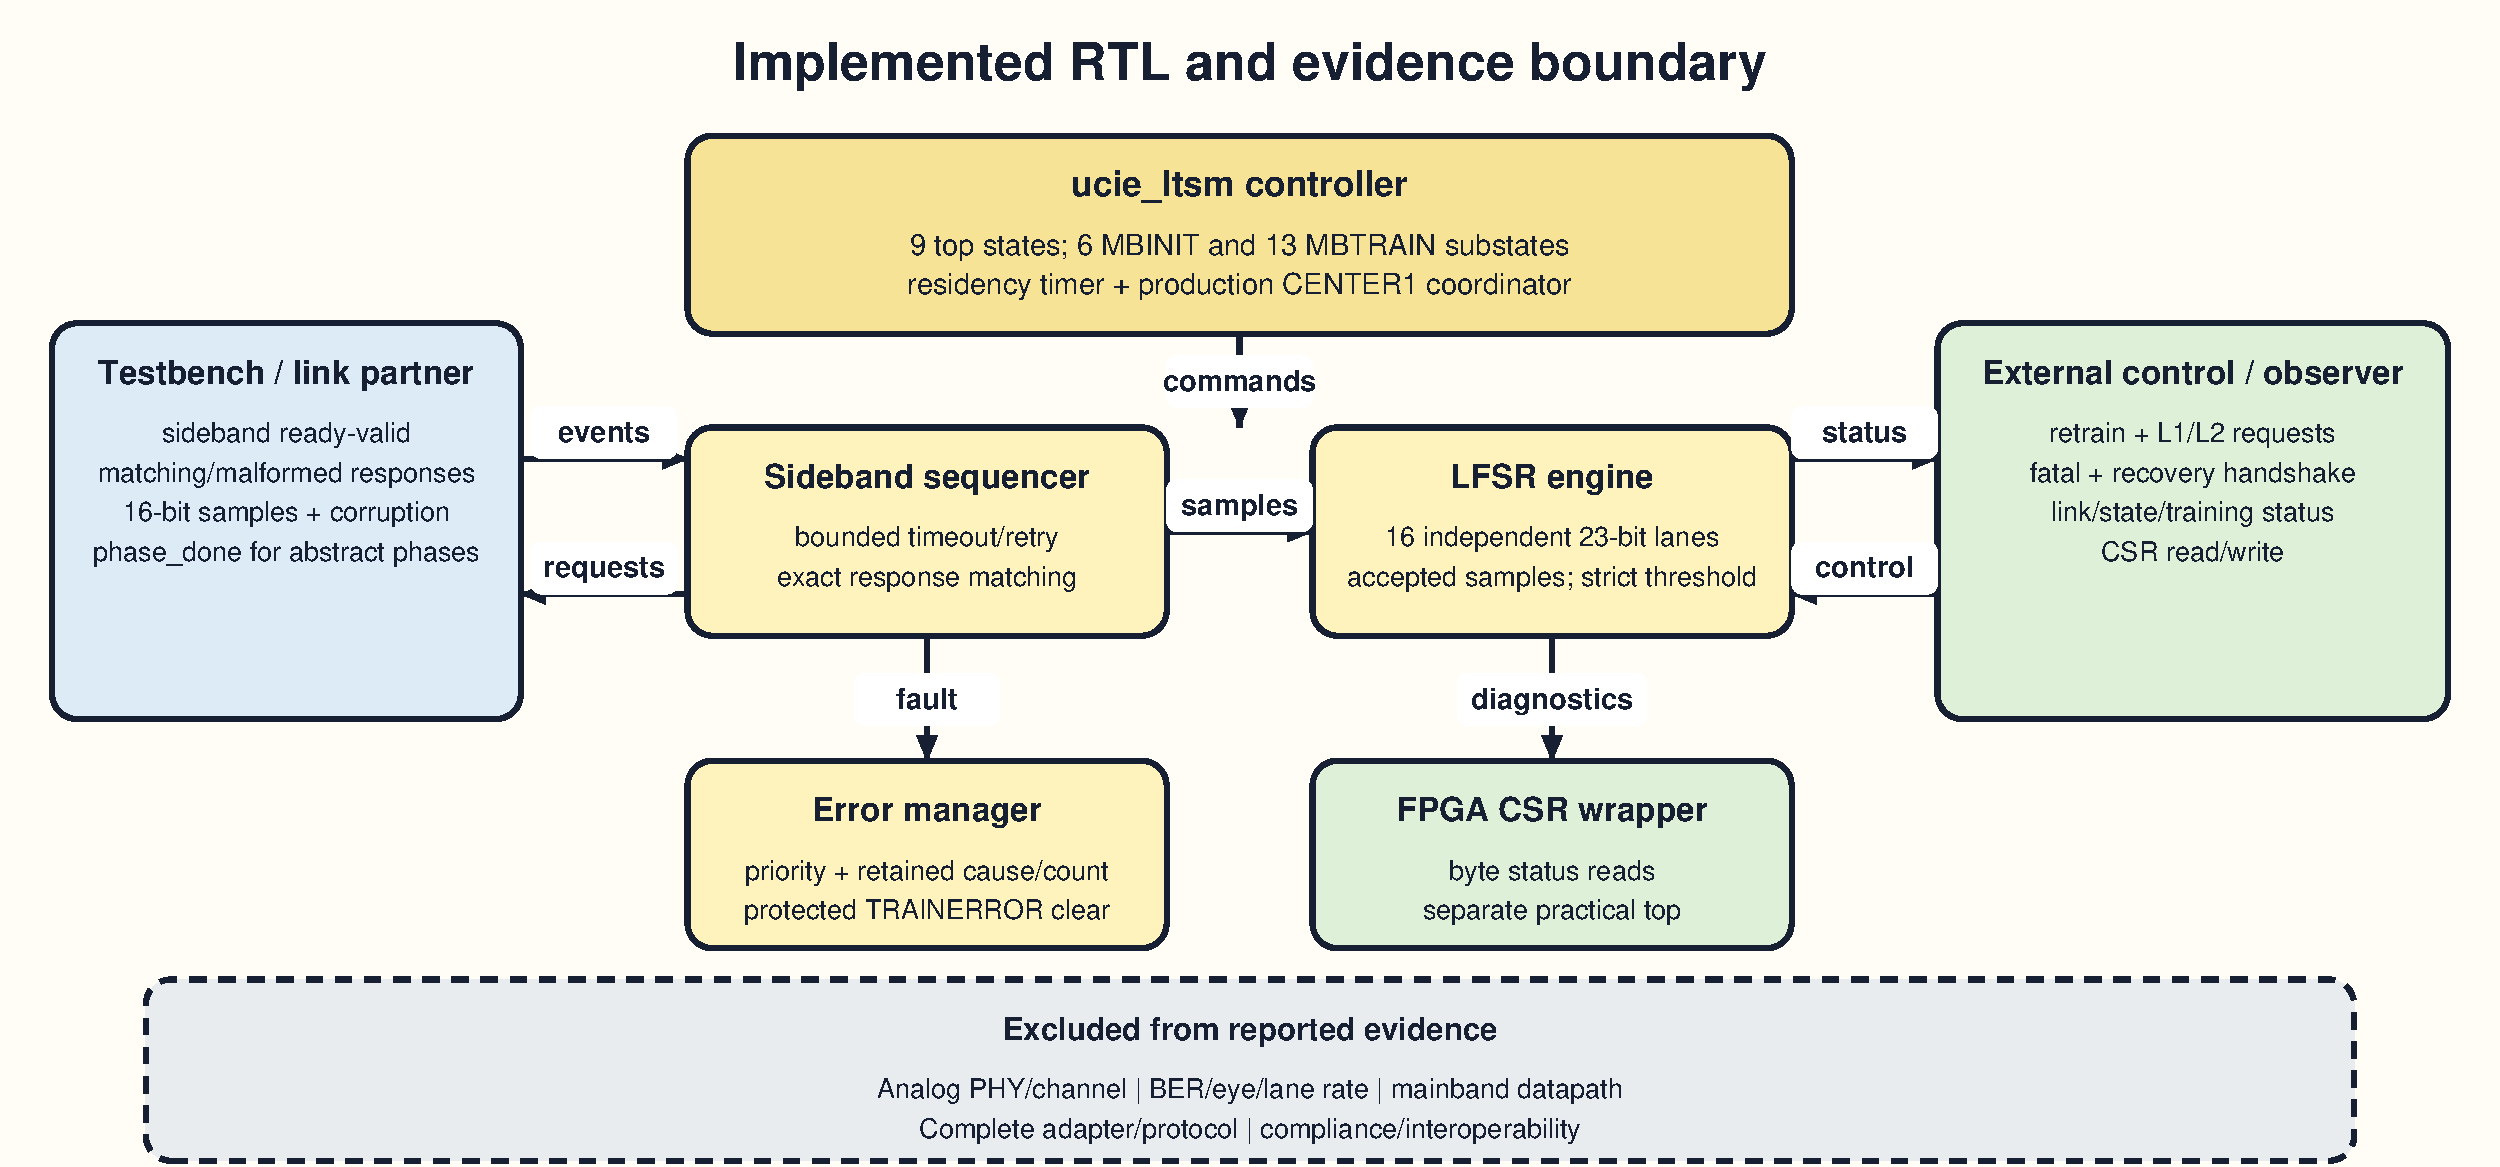
\includegraphics[width=0.97\textwidth]{fig01_scope.pdf}
\caption{Implemented RTL and evidence boundary. Colored blocks identify the
synthesized modules and their test/observer interfaces; the pale dashed panel
lists excluded physical-layer and full-protocol functions.}
\label{fig:scope}
\end{figure*}

The modeled state and substate names follow UCIe Specification Revision 2.0,
Version 1.0 \cite{ucie20}. Most MBINIT, MBTRAIN, and PHYRETRAIN operations are
represented by an external \texttt{phase\_done\_i} condition. One training
operation, DATATRAINCENTER1, is implemented through the sideband and LFSR
engines. The distinction prevents a control-flow model from being mistaken for
a complete PHY.

\subsection{Module Decomposition}

Fig.~\ref{fig:rtl} shows the synthesizable hierarchy. The top-level
\texttt{ucie\_ltsm} owns state/substate registers, a residency timer, routing,
and engine coordination. Three engines isolate operations whose temporal
contracts differ from ordinary state progression.

\begin{figure*}[t]
\centering
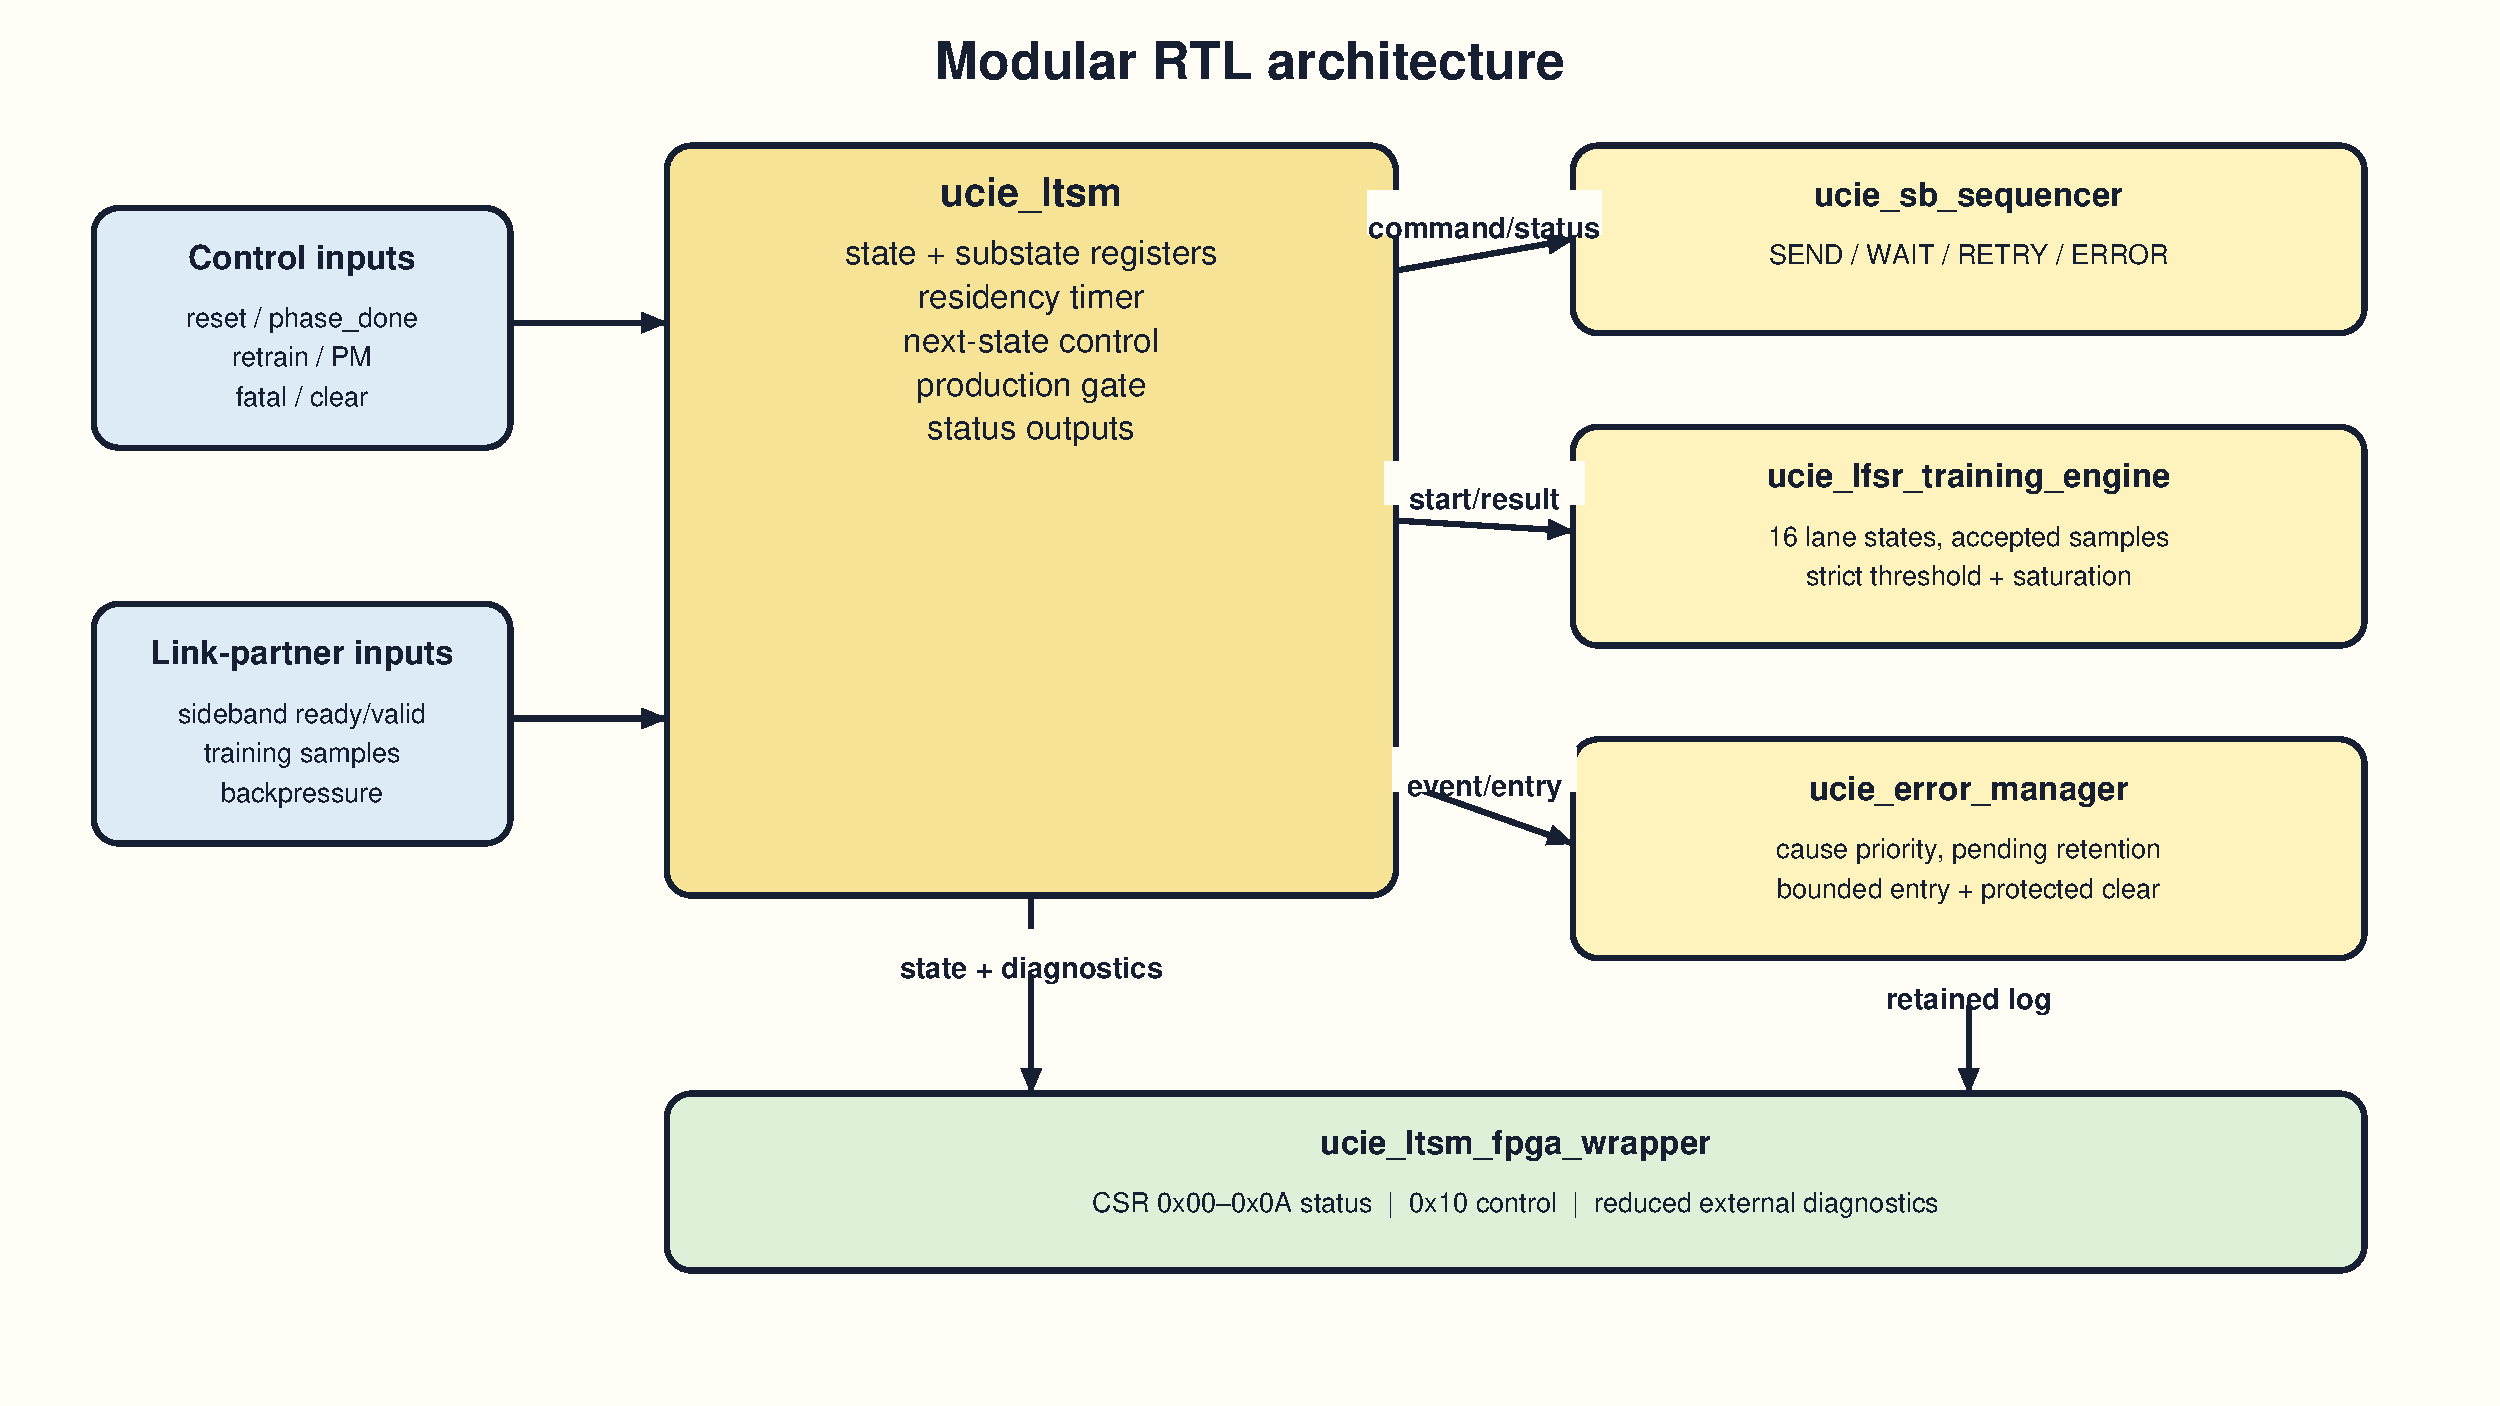
\includegraphics[width=0.96\textwidth]{fig02_rtl_architecture.pdf}
\caption{Synthesizable hierarchy. The controller instantiates the sideband,
LFSR, and error engines. The separate FPGA top instantiates the same controller
and serializes its wide diagnostics through a compact CSR interface.}
\label{fig:rtl}
\end{figure*}

The sideband sequencer has IDLE, SEND, WAIT, and ERROR states. It holds the
request under ready/valid backpressure, accepts only the expected response,
retries a bounded number of response timeouts, and exposes protocol error and
abort status. The current message enumeration includes NOP, SBINIT-DONE
request/response, and DATACENTER1 START/END request/response. It is not a
complete sideband packet layer.

The LFSR engine maintains 16 independent 23-bit states. Eight nonzero seeds are
repeated over the lanes, and the feedback polynomial is
$x^{23}+x^{21}+x^{16}+x^8+x^5+x^2+1$. State and sample count advance only when
\texttt{train\_rx\_valid\_i} accepts a sample. Mismatches accumulate in a
16-bit saturating counter, and pass is asserted only when the final count is
strictly less than the programmed threshold; equality fails. Fig.~\ref{fig:lfsr}
summarizes the datapath and its independent reference boundary.

\begin{figure*}[t]
\centering
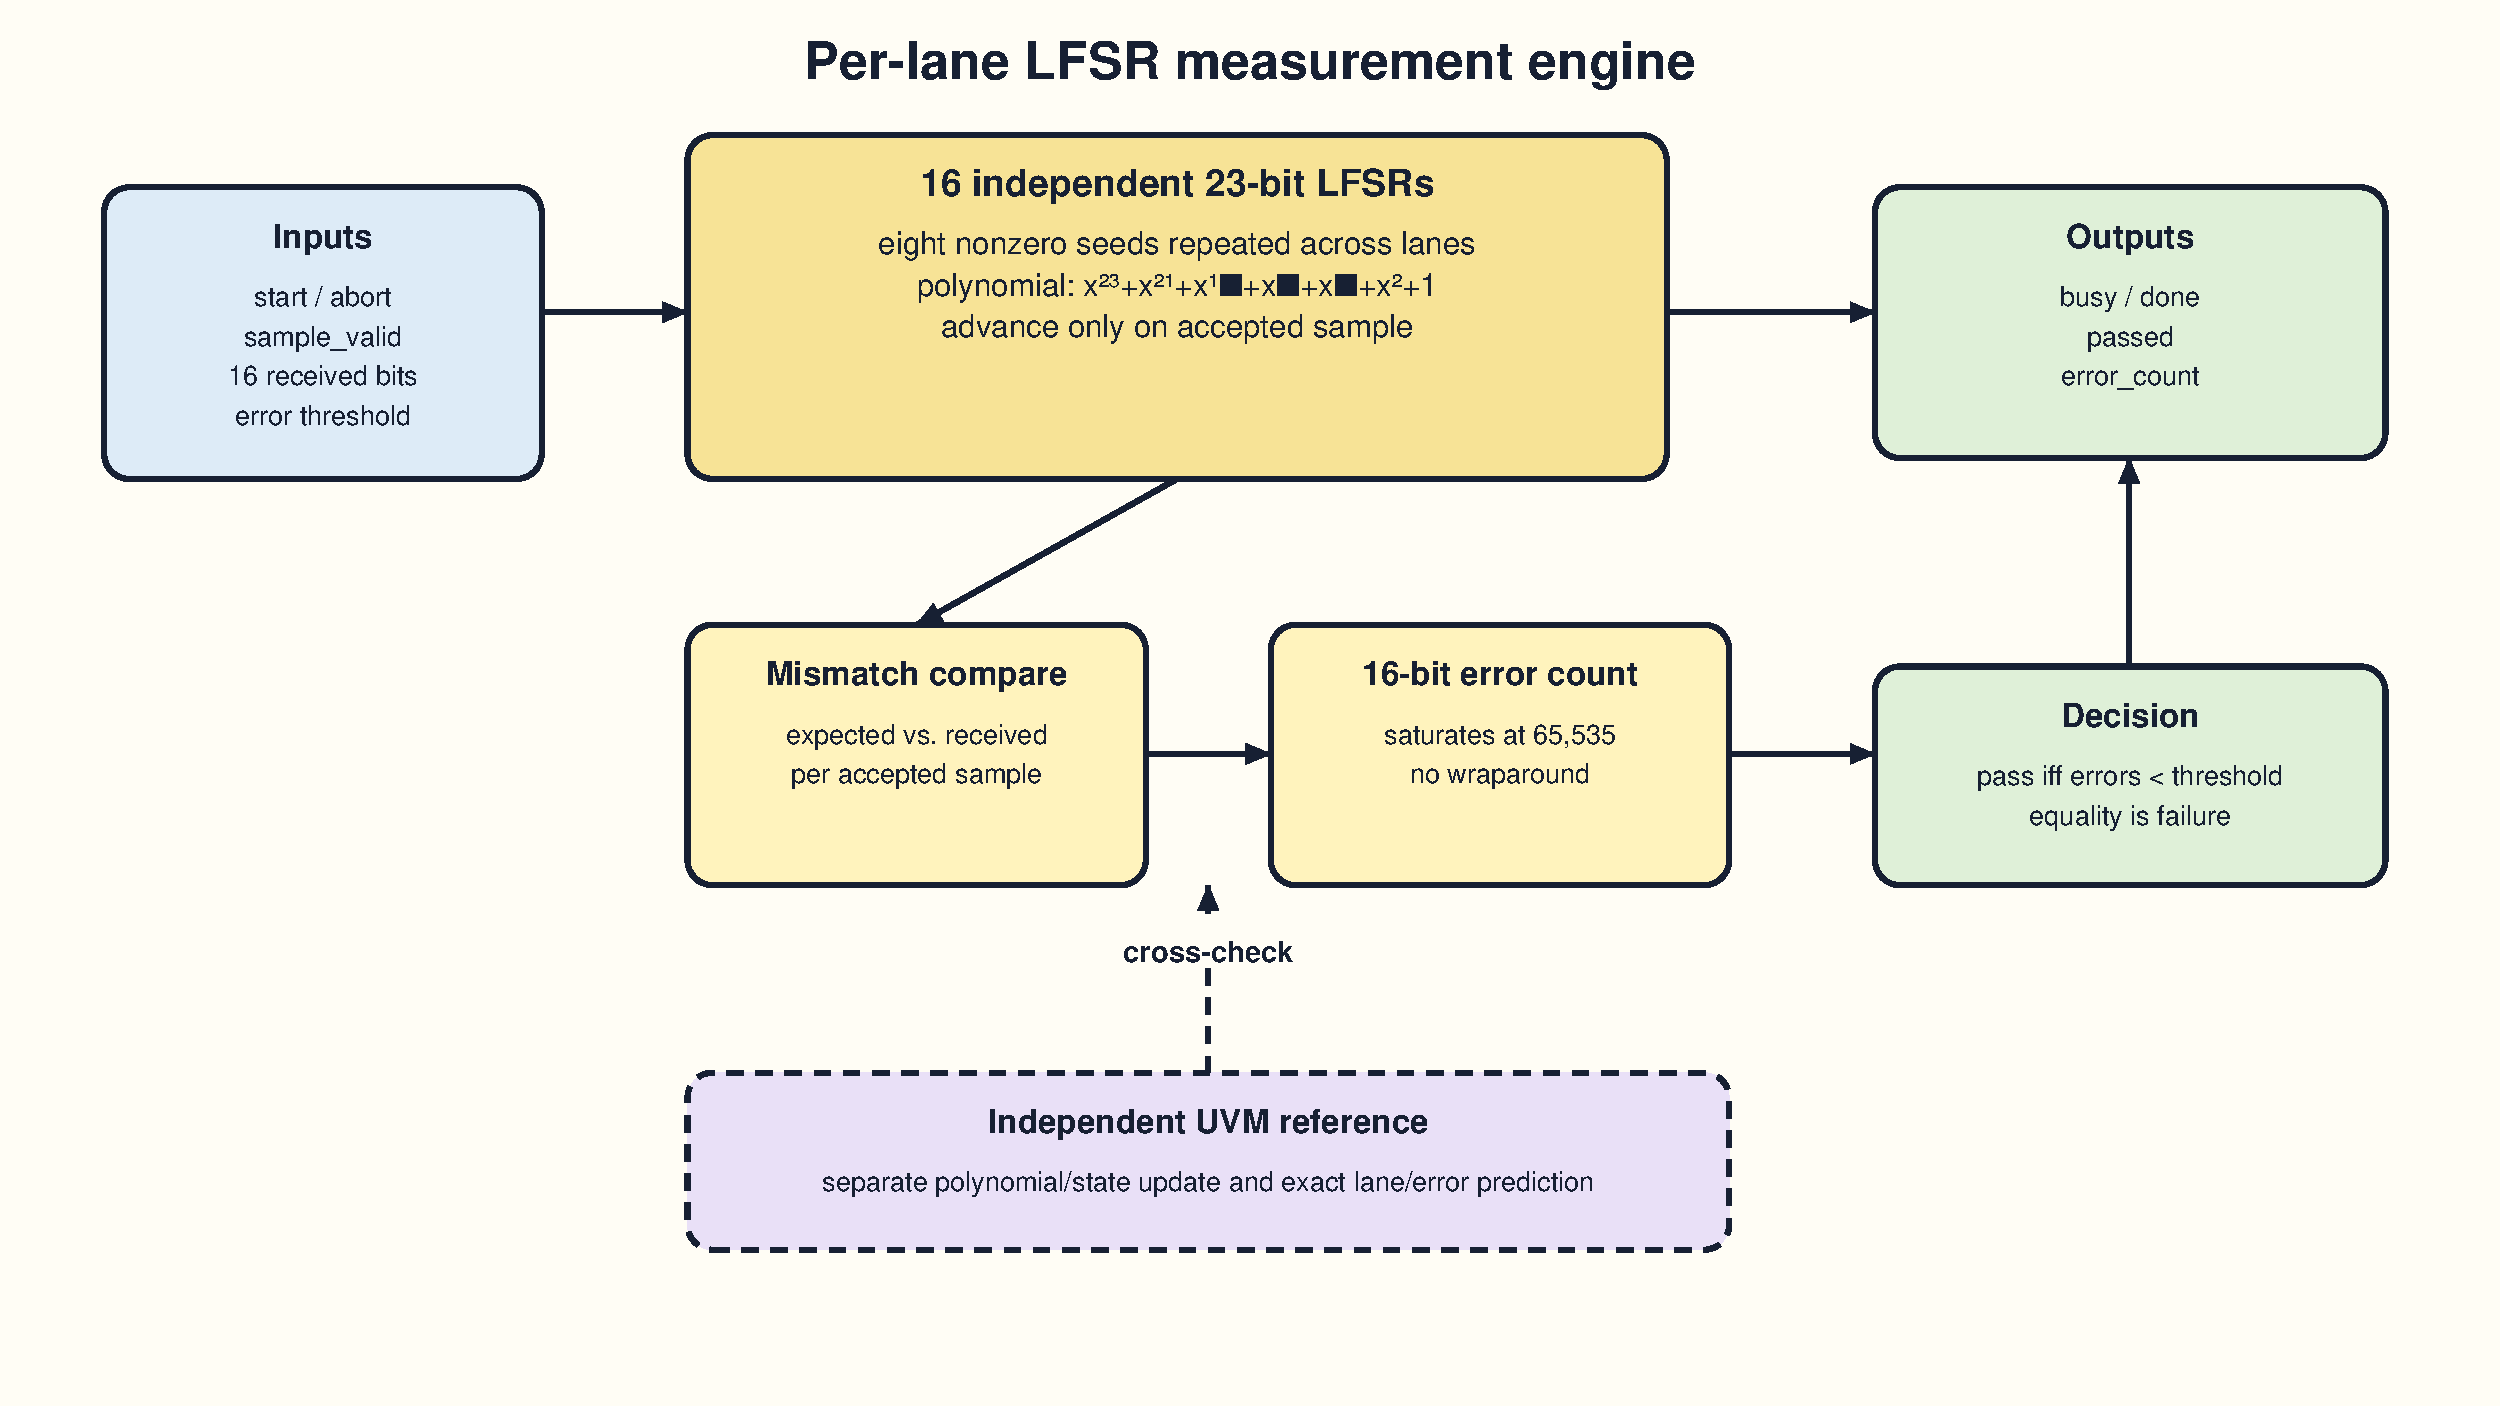
\includegraphics[width=0.86\textwidth]{fig05_lfsr_engine.pdf}
\caption{LFSR measurement engine. Receive gaps freeze both the sample count and
per-lane expected state.}
\label{fig:lfsr}
\end{figure*}

Fig.~\ref{fig:wave-lfsr} is a VCD-backed module-directed capture rather than a
hand-drawn timing sketch. The receive-valid gaps leave the expected lane state
and error count unchanged; the accepted TX/RX samples match, so the engine
asserts done and pass after the eighth accepted sample. Signal names in the
standalone SVG link to the repository's public
\href{https://github.com/Varadain/ucie-ltsm/blob/feature/v1.0-integrated-training/docs/02_ltssm/signals.md}{signal-definition guide}.

\begin{figure*}[t]
\centering
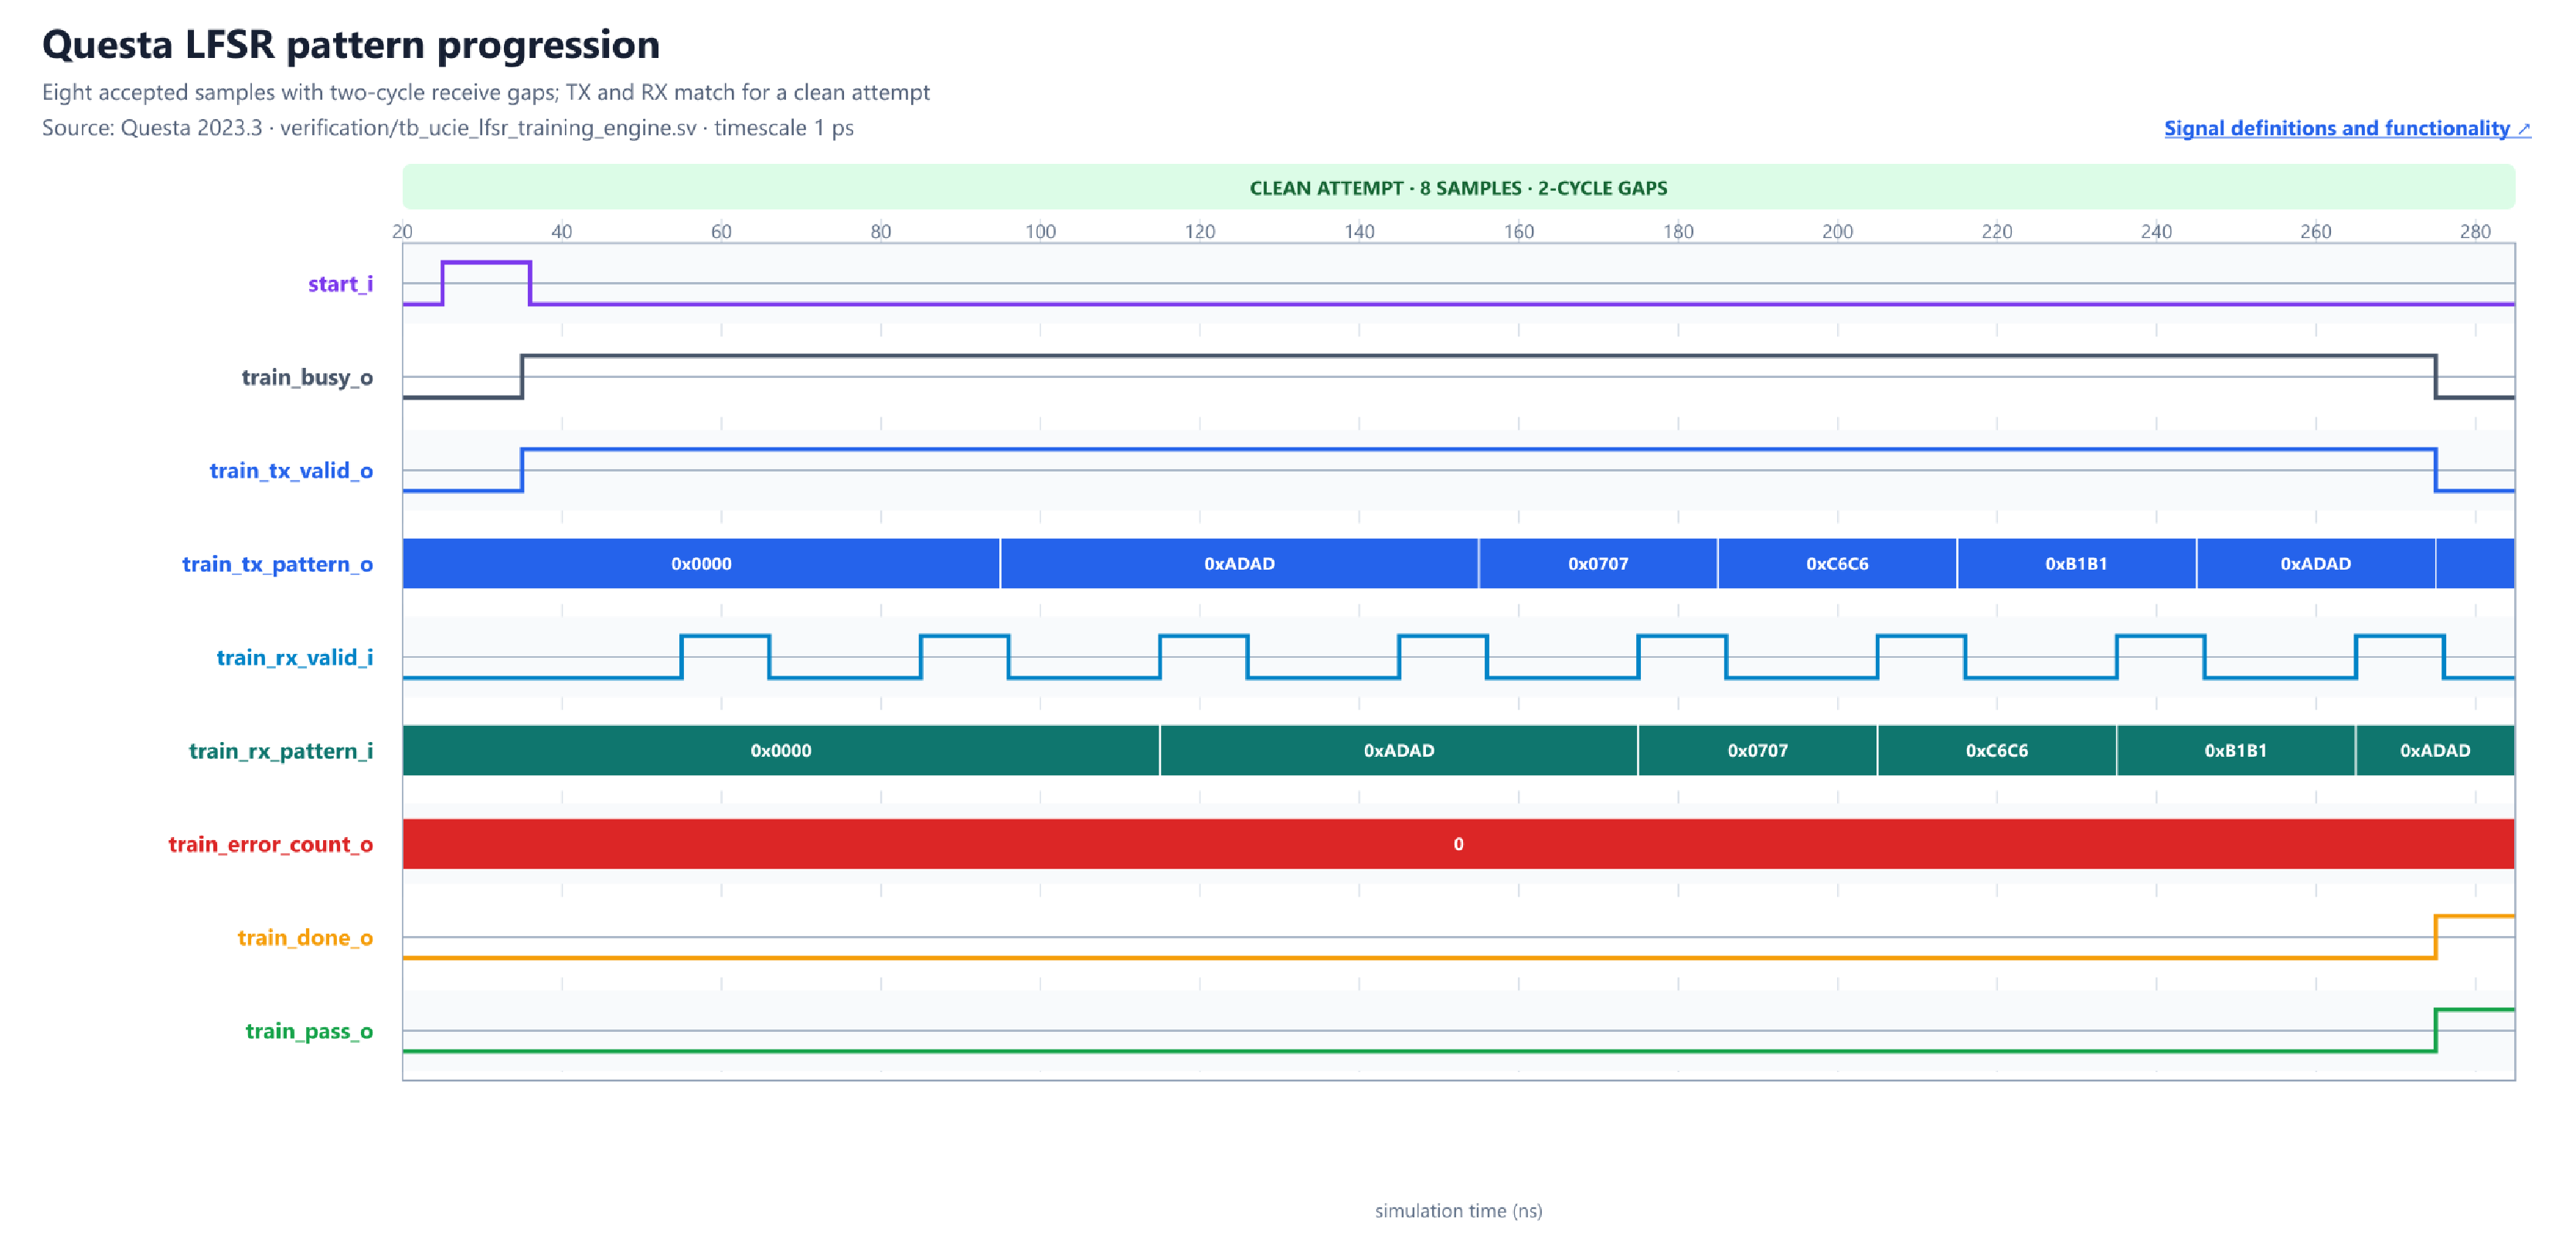
\includegraphics[width=0.97\textwidth]{fig09_wave_lfsr.pdf}
\caption{Color-coded Questa waveform generated from
\texttt{build/waves/datatrain\_lfsr.vcd}. The capture shows sample-gated LFSR
progression, an exact zero mismatch count, and the final done/pass decision.}
\label{fig:wave-lfsr}
\end{figure*}

The error manager accepts one eligible state-timeout, sideband-protocol, or
local-fatal event. Simultaneous events use the fixed priority timeout,
sideband, then fatal. A pending event holds the TRAINERROR request until an
acknowledgment or manager timeout permits entry. Cause and a saturating 16-bit
event count remain stable in TRAINERROR. A software clear is accepted only
when no event is pending and the controller is outside TRAINERROR.

\subsection{Hierarchical LTSM Control}

The package enumerates nine top states: RESET, SBINIT, MBINIT, MBTRAIN,
LINKINIT, ACTIVE, PHYRETRAIN, TRAINERROR, and L1/L2. MBINIT contains six
substates and MBTRAIN contains thirteen. The nominal route progresses through
initialization and training to ACTIVE. From ACTIVE, requests can select one of
three retraining targets or enter the modeled low-power state; exit conditions
return to ACTIVE. Eligible timeout, protocol, or fatal conditions route through
the retained error manager to TRAINERROR, as shown in
Fig.~\ref{fig:ltsmflow}.

\begin{figure*}[t]
\centering
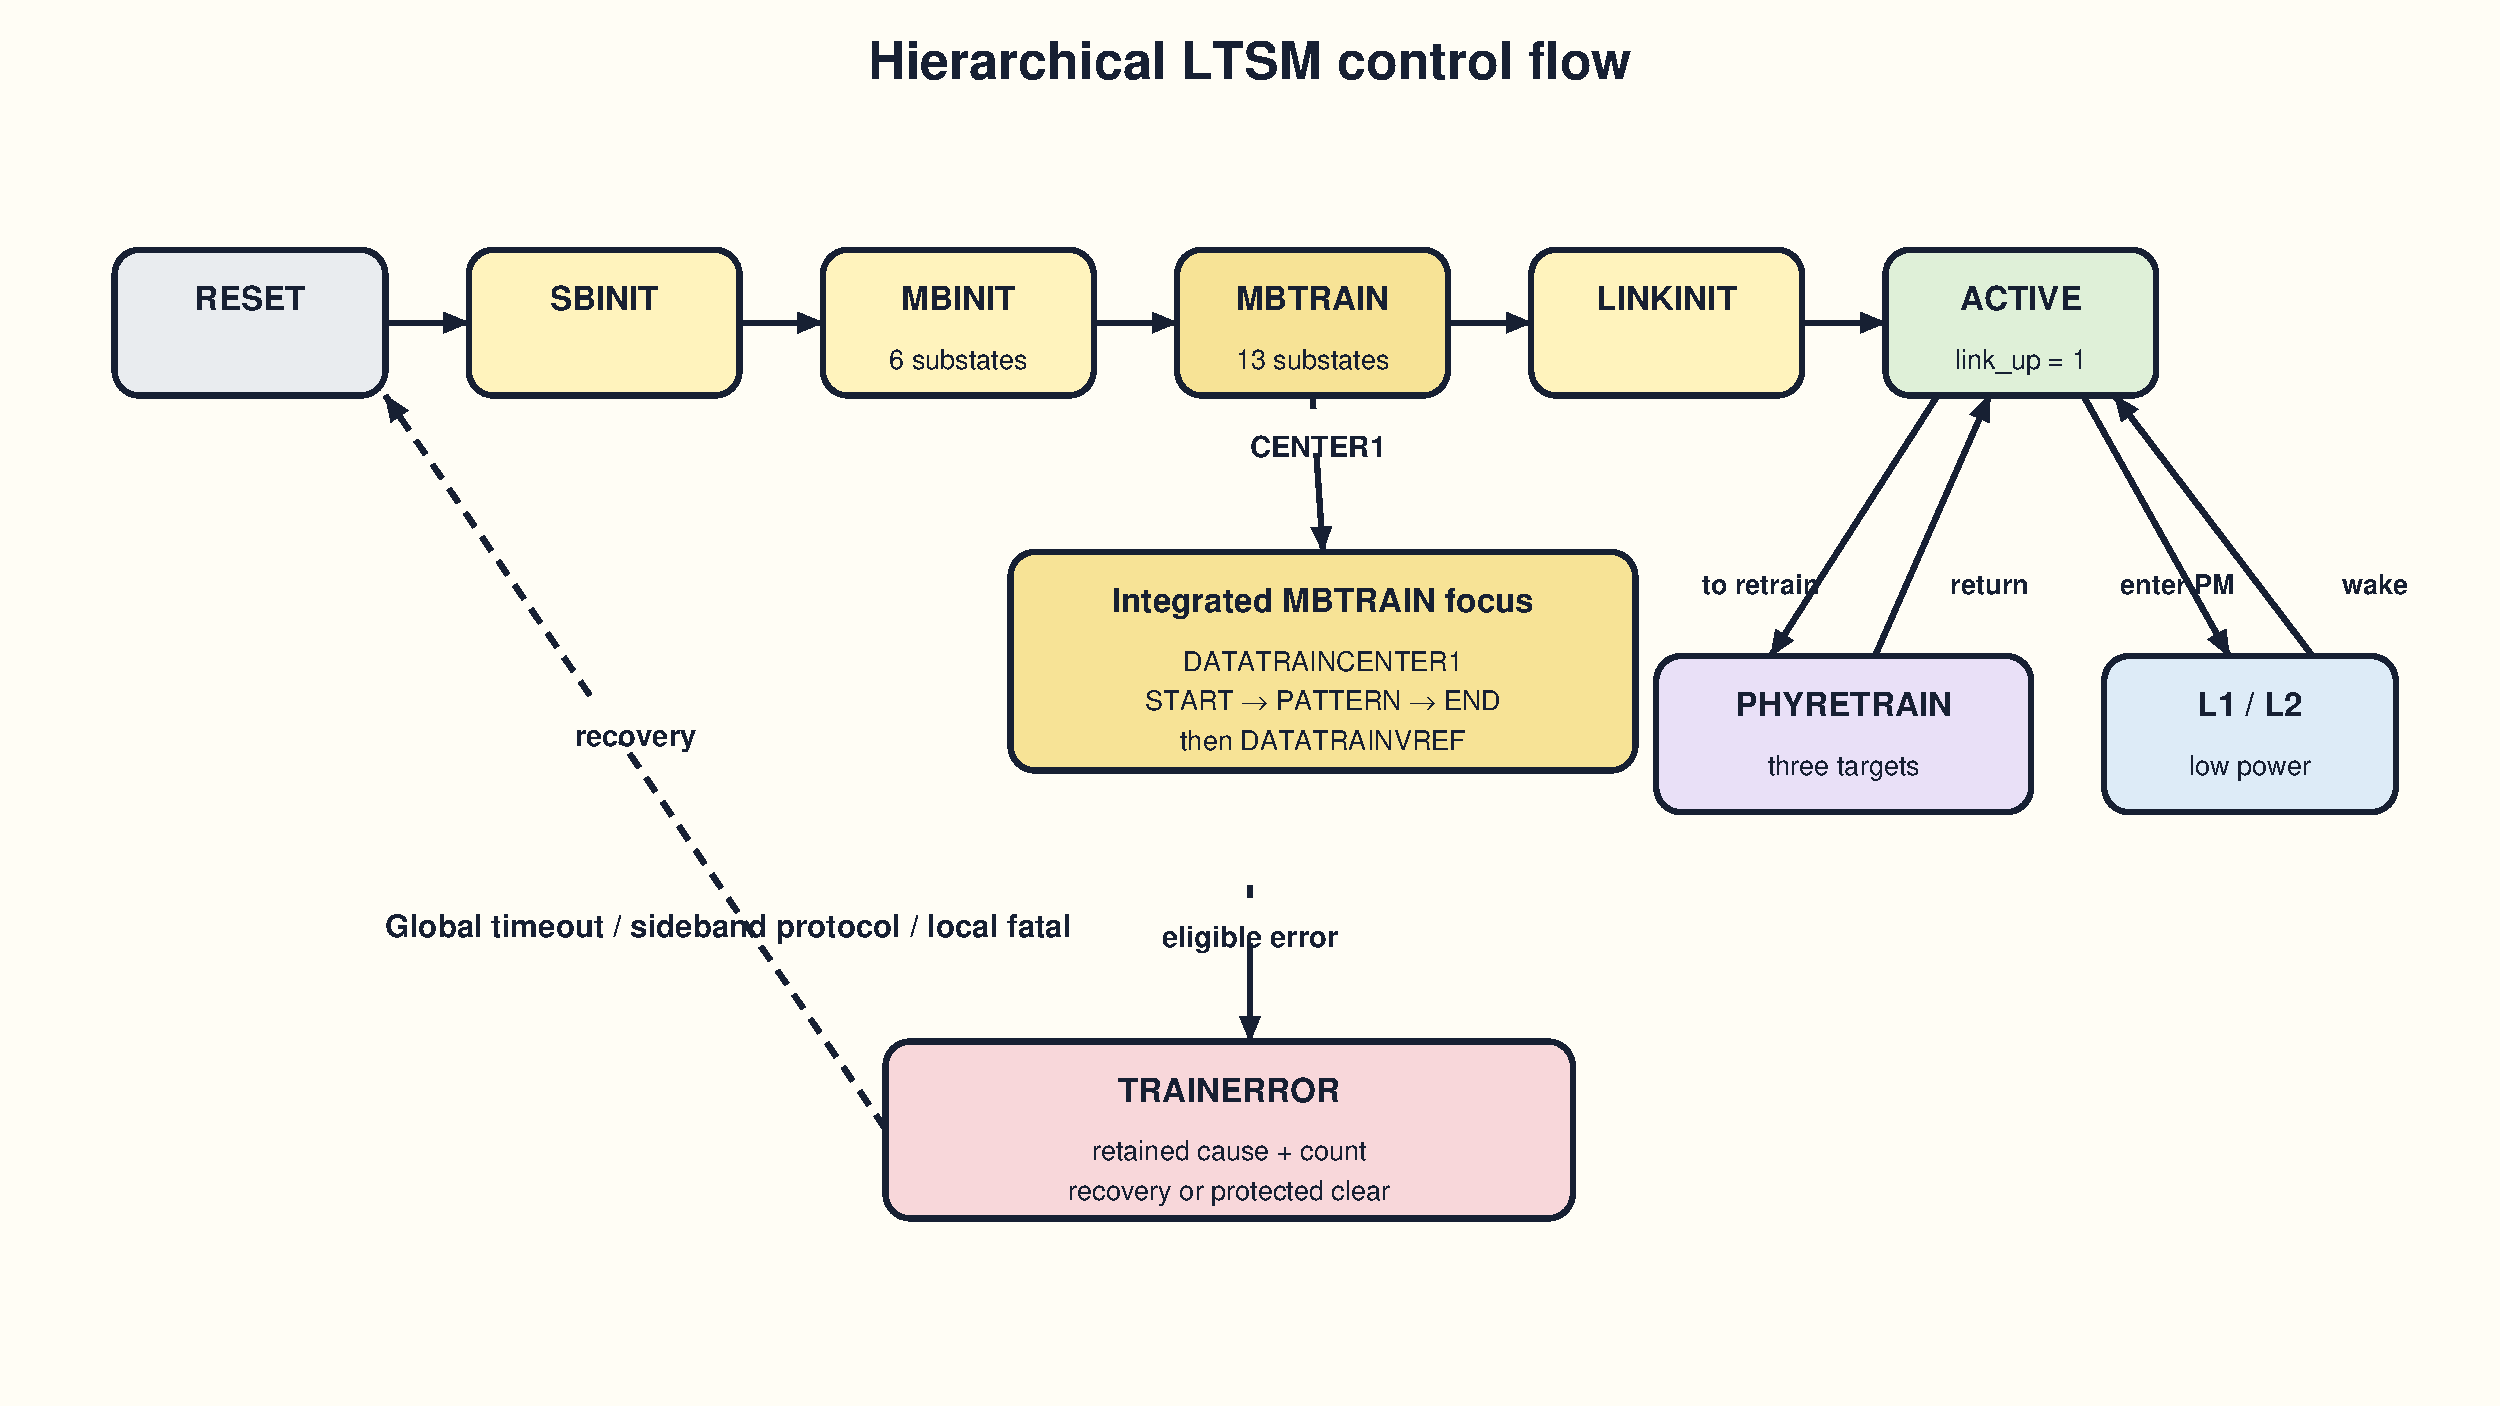
\includegraphics[width=0.93\textwidth]{fig03_ltsm_flow.pdf}
\caption{Hierarchical controller flow. Only DATATRAINCENTER1 is expanded here;
other physical operations remain phase-completion abstractions.}
\label{fig:ltsmflow}
\end{figure*}

One timer measures state/substate residency. It restarts on a state or substate
change and can be stalled by the environment. Default parameters correspond to
an 80-MHz controller clock, a 4-ms reset interval, an 8-ms residency timeout,
a 256-cycle sideband response timeout, one retry, and 4096 training samples.
Testbenches scale selected values for runtime while retaining the ordering
properties under test.

\subsection{Integrated DATATRAINCENTER1 Protocol}

Production mode fixes the abstract CENTER1 bypass to zero. On entering
DATATRAINCENTER1, the controller orders the sideband engine to send START and
wait for its matching response. Only then may the LFSR engine begin. A failed
pattern re-enters the pattern phase without emitting END; a passing pattern
starts the END exchange. Advancement to DATATRAINVREF requires the matching END
response. A mismatch, exhausted sideband retry, fatal event, state timeout, or
reset aborts the sequence along its corresponding control path.

\begin{figure*}[t]
\centering
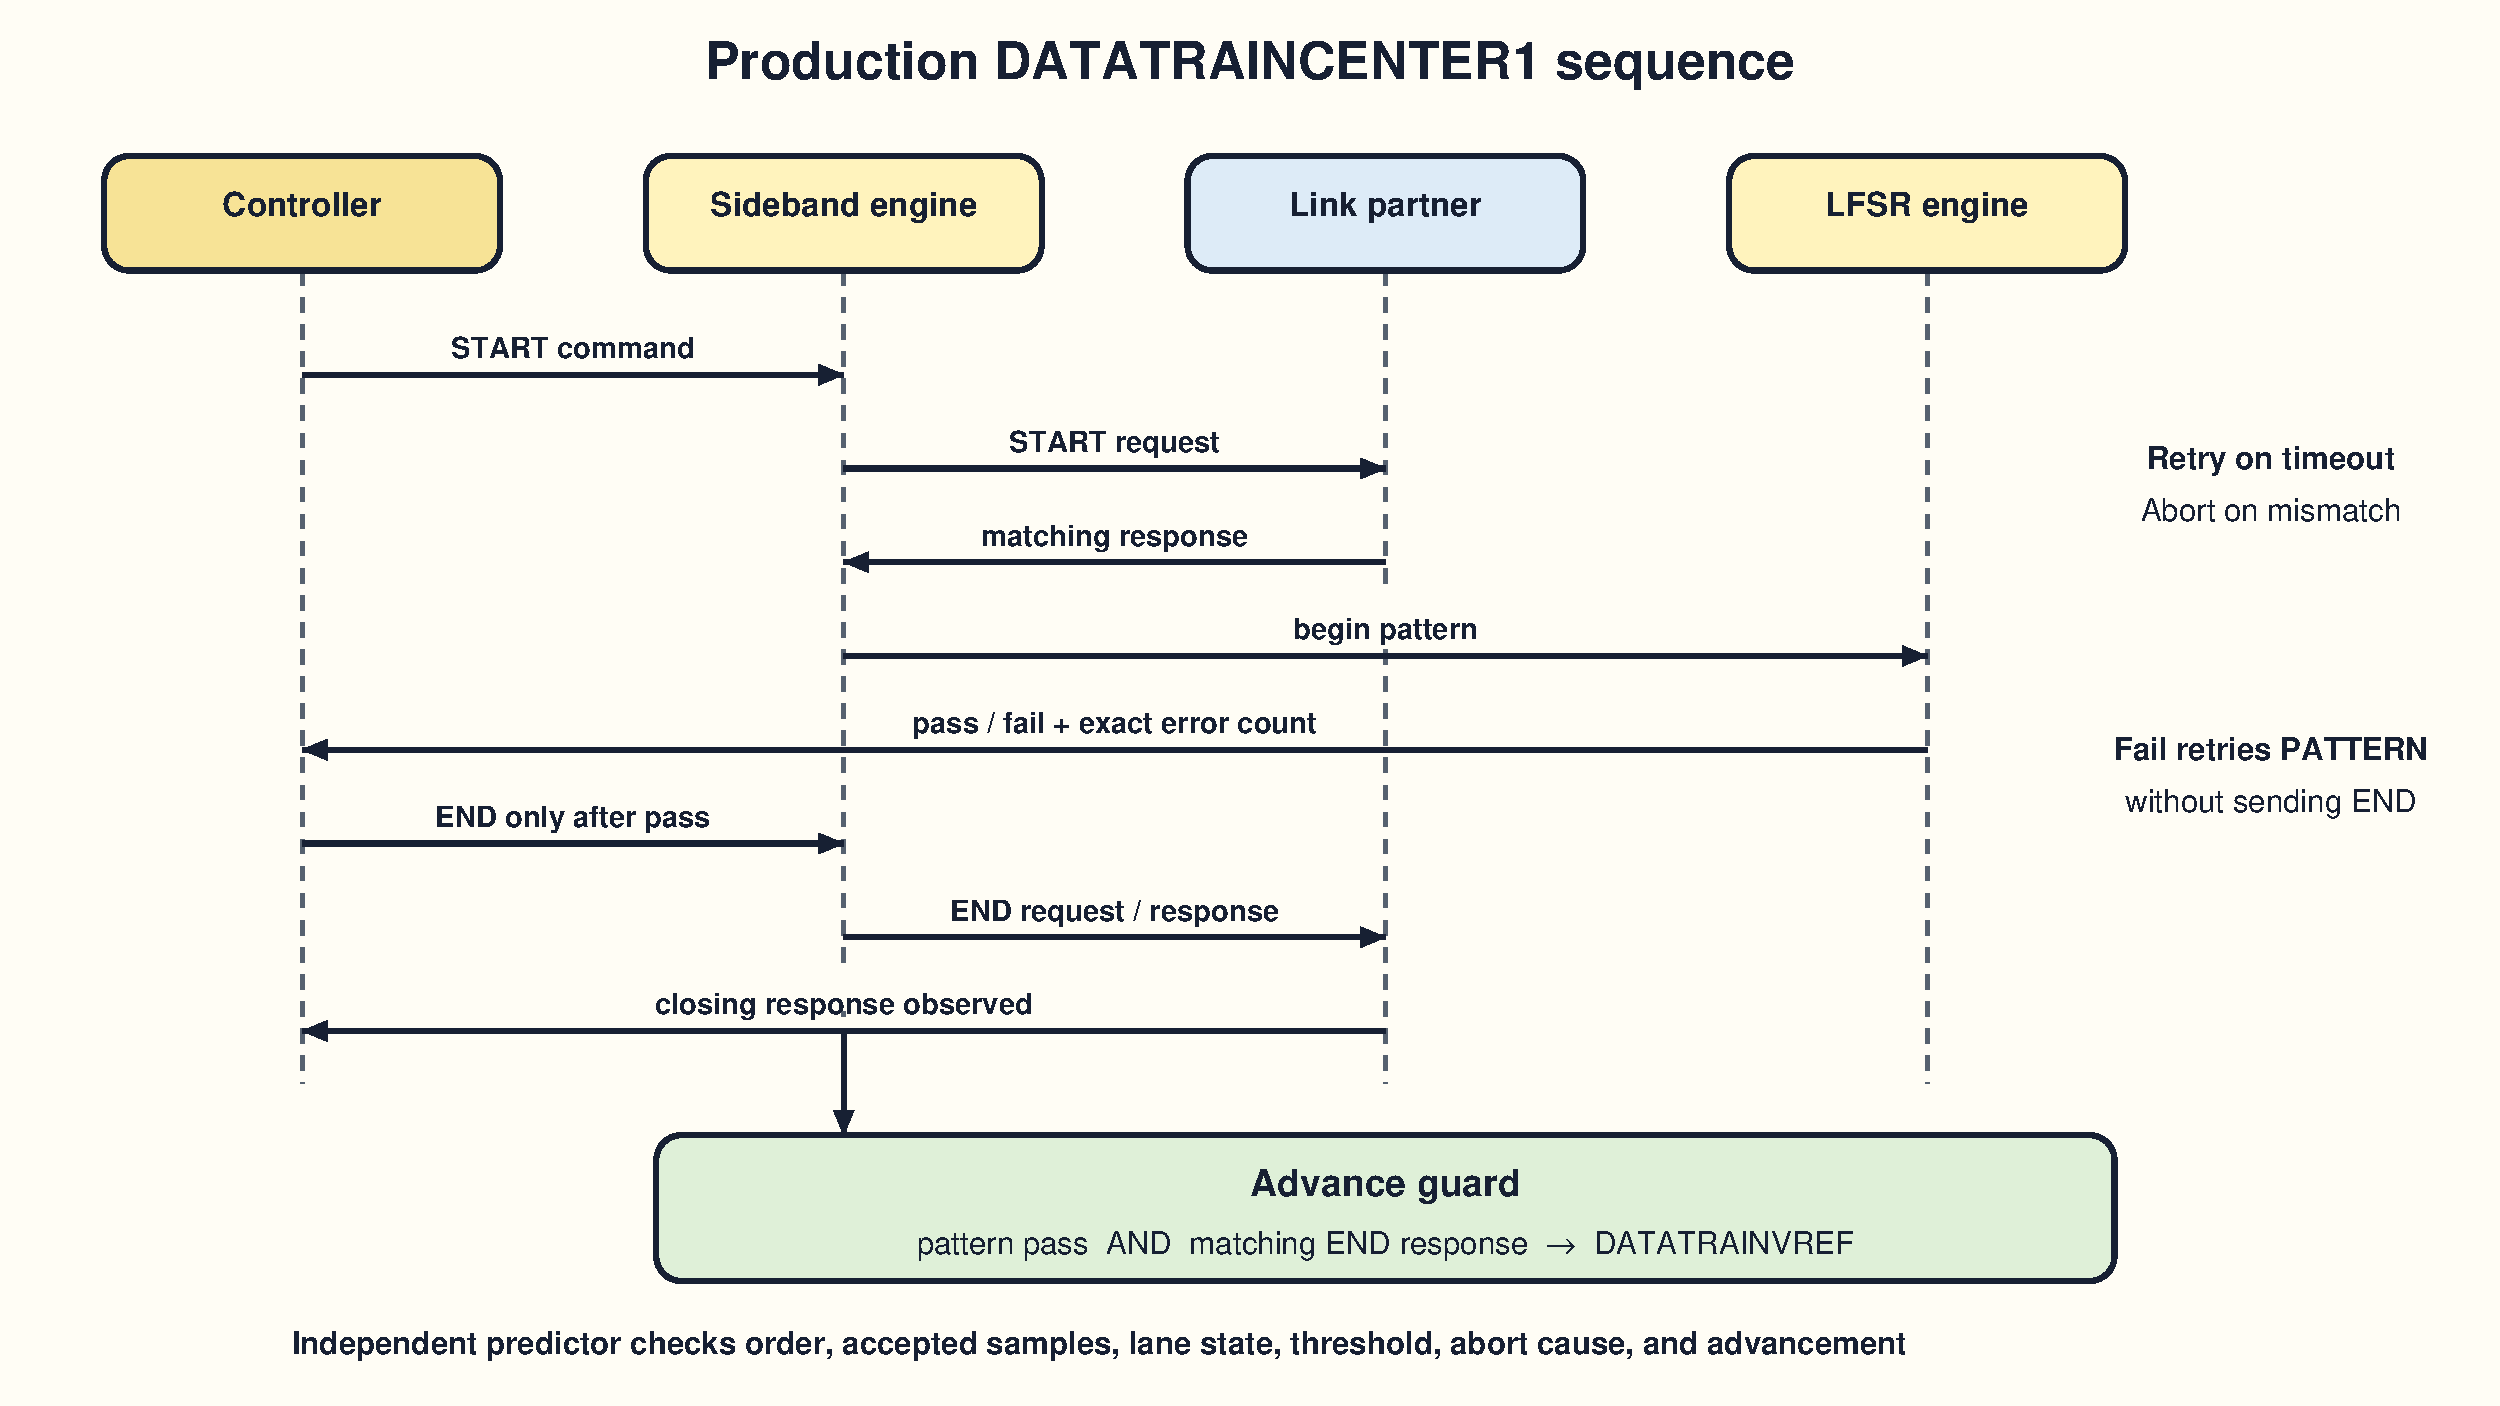
\includegraphics[width=0.93\textwidth]{fig04_integrated_sequence.pdf}
\caption{Integrated CENTER1 transaction order. The independent predictor checks
the same interface events without reading the DUT's private LFSR state.}
\label{fig:center1}
\end{figure*}

This ordering, illustrated in Fig.~\ref{fig:center1}, creates two explicit
commit barriers: the START response admits pattern activity, and the END
response admits state advancement. Separating the sideband and pattern engines
keeps retry time from advancing training state and keeps receive gaps from
consuming the sideband timeout counter.

\subsection{Retained Diagnostics and FPGA CSR}

The compact wrapper preserves the controller interface internally but replaces
wide state/error/training diagnostics with byte reads. Read addresses 0x00,
0x01, and 0x02 expose top, MBINIT, and MBTRAIN state; 0x03 exposes status bits;
0x04 exposes error cause; 0x05--0x06 and 0x07--0x08 expose retained-event and
training-error counts; 0x09 returns version 0x04; and 0x0A exposes the integrated
training phase. Writing bit 0 at 0x10 requests a protected log clear. Undefined
reads return zero.

Fig.~\ref{fig:recovery} connects the retained log, entry handshake, recovery
route, CSR view, and assertion boundary. This observability choice is not only
documentation convenience: Sec.~\ref{sec:evaluation} shows that exporting wide
diagnostics prevents the chosen FPGA from fitting, whereas the CSR wrapper
fits.

\begin{figure*}[t]
\centering
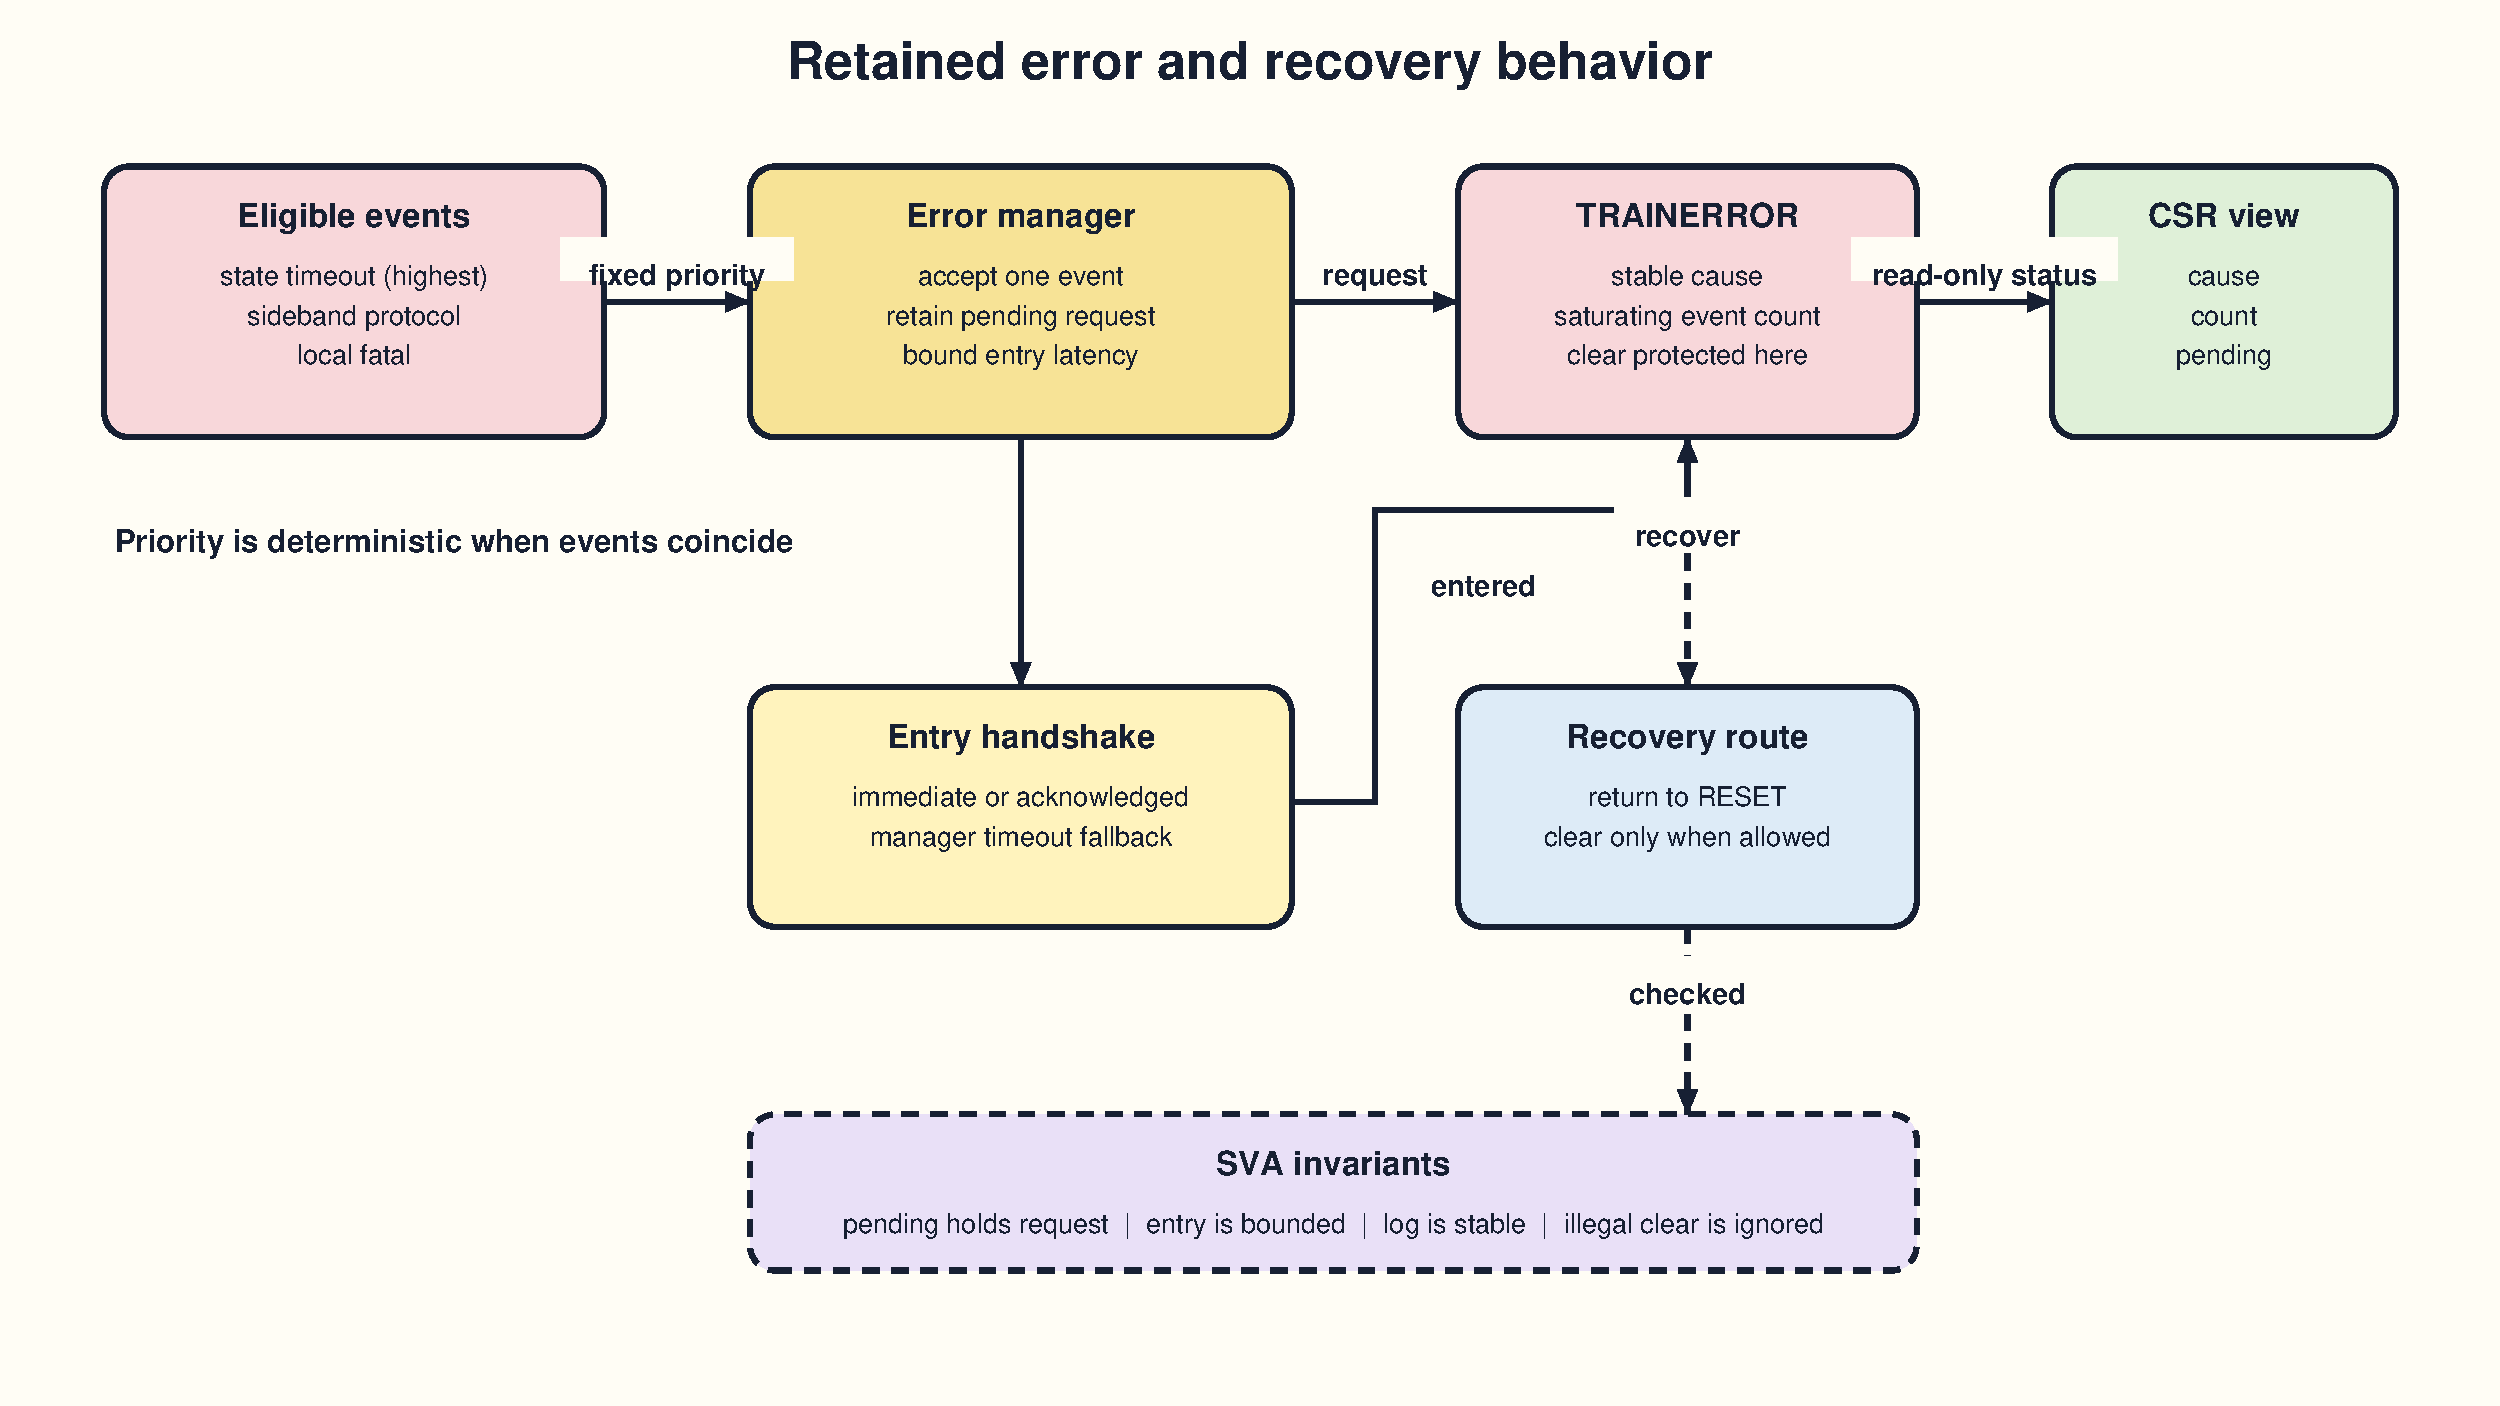
\includegraphics[width=0.86\textwidth]{fig06_error_recovery.pdf}
\caption{Retained error and recovery flow. Clear is ignored while an event is
pending or the state is TRAINERROR.}
\label{fig:recovery}
\end{figure*}

The VCD-backed capture in Fig.~\ref{fig:wave-error} makes the temporal contract
visible. A one-cycle fatal event is retained, the request remains asserted
while pending, and a clear attempt is ignored before the bounded TRAINERROR
entry. The retained cause and event count survive until recovery reaches an
eligible clear state.

\begin{figure*}[t]
\centering
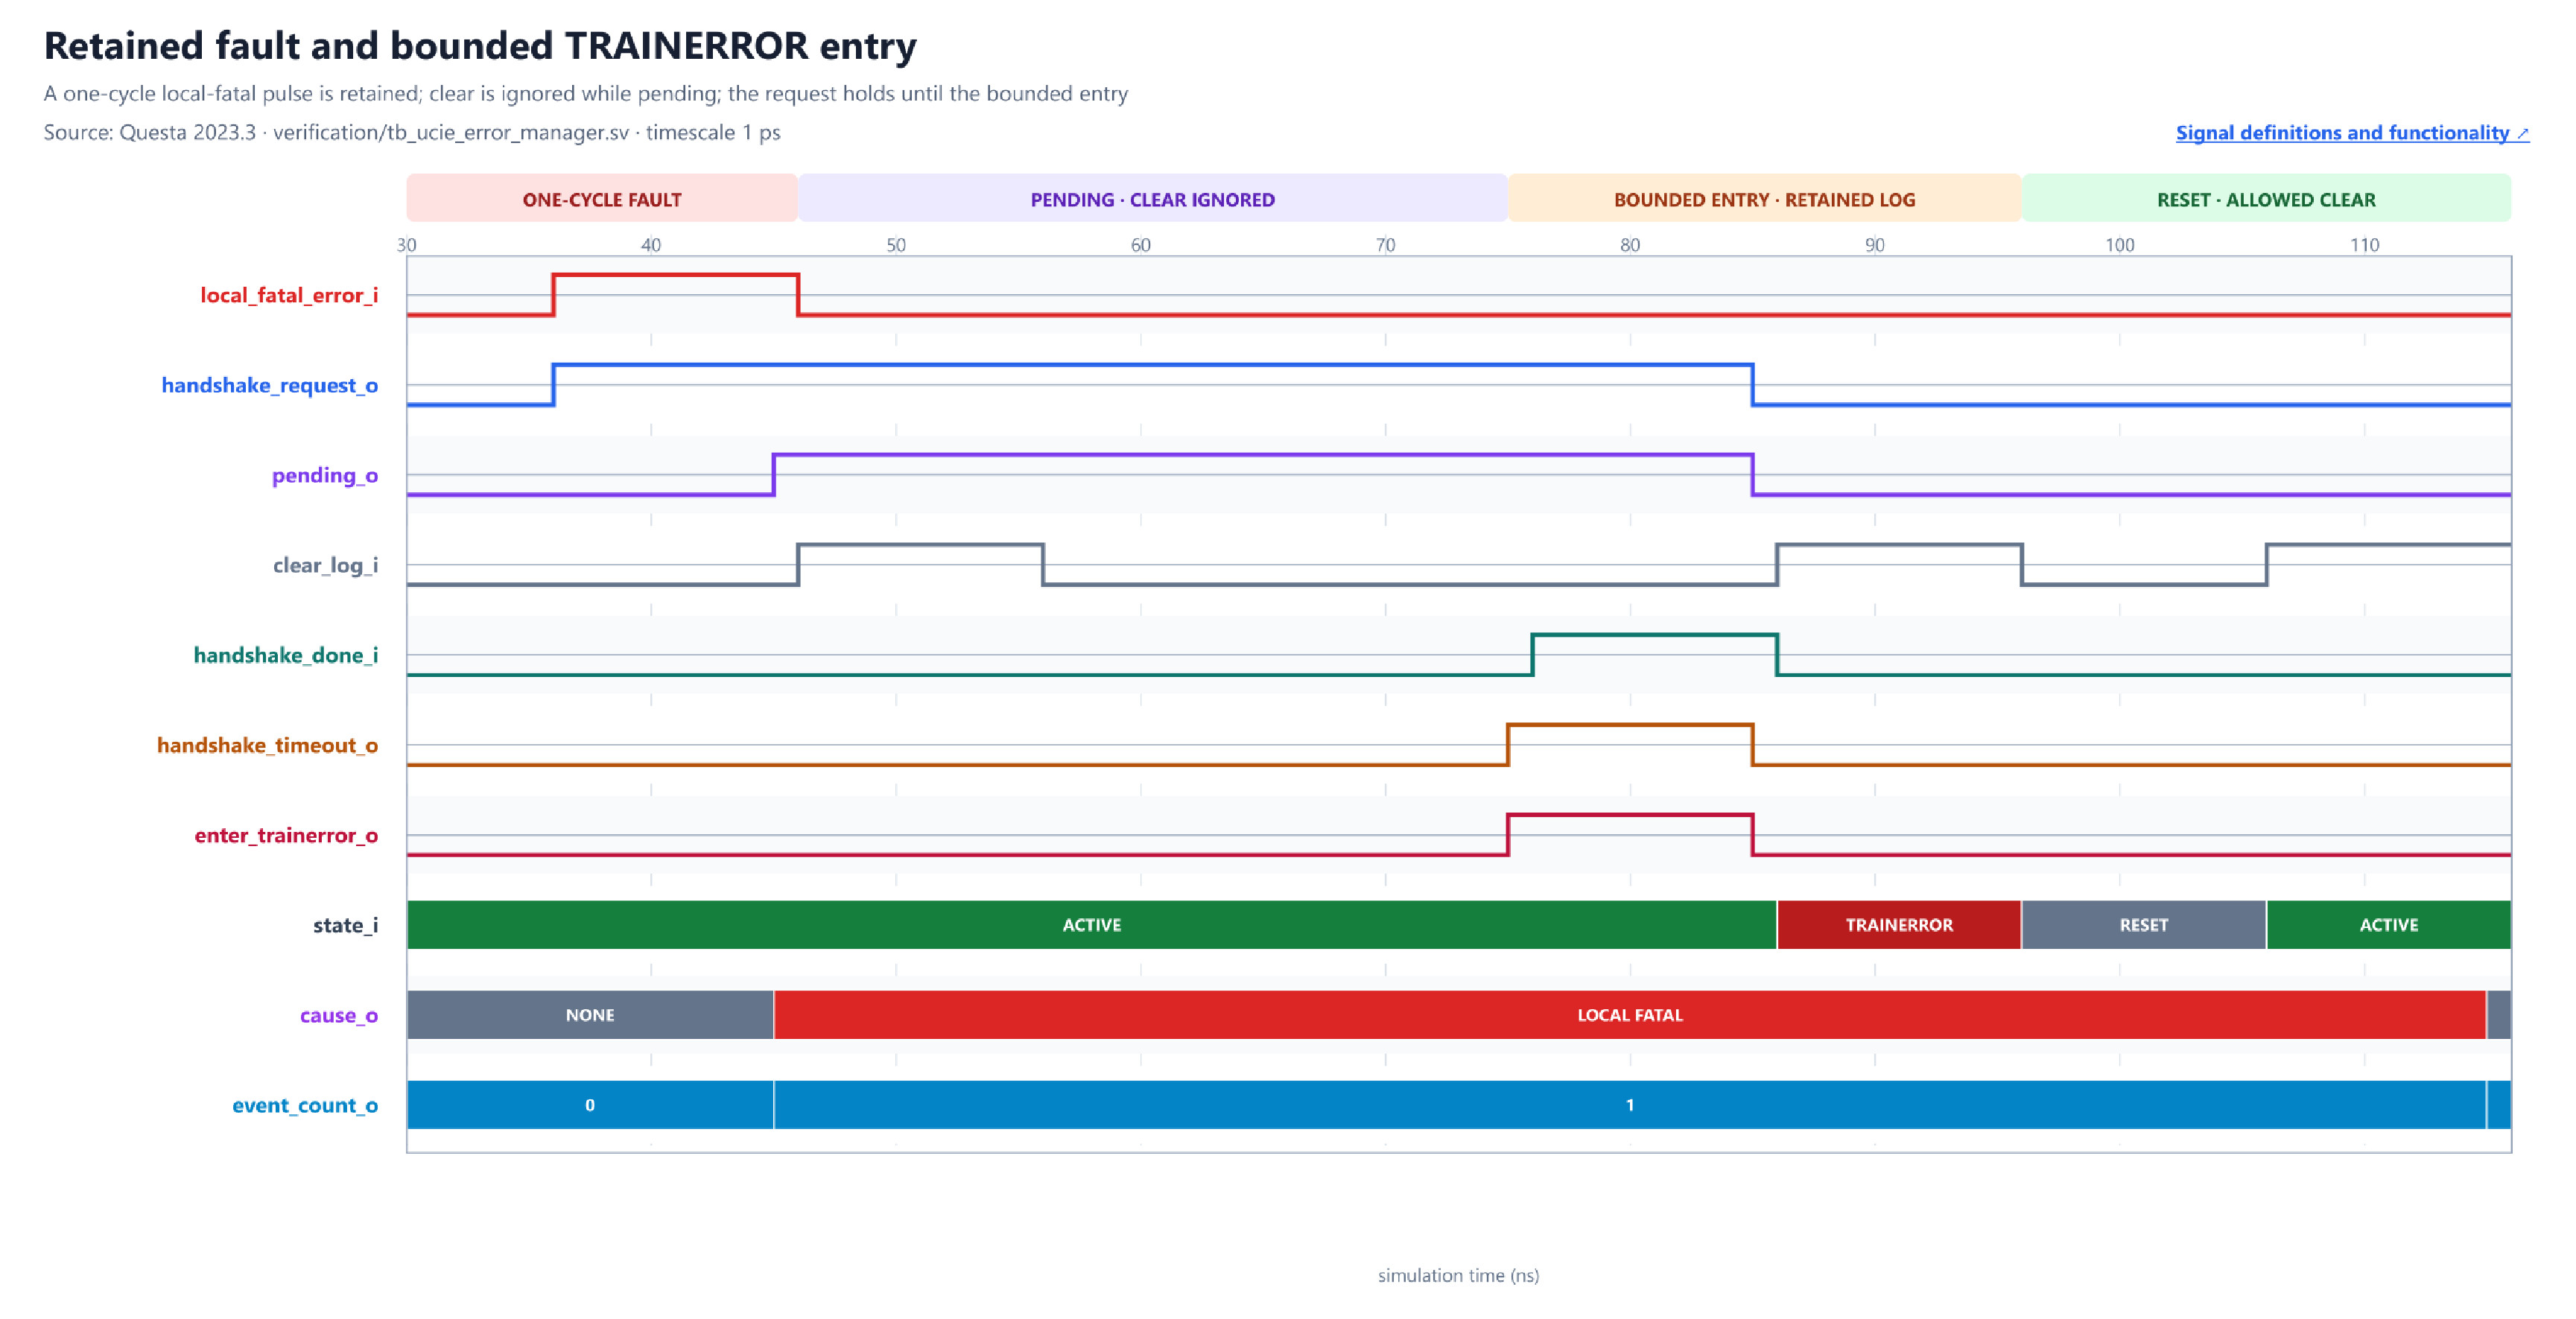
\includegraphics[width=0.97\textwidth]{fig10_wave_trainerror.pdf}
\caption{Color-coded Questa waveform from the self-checking error-manager
testbench. Colored phase bands identify fault capture, protected pending time,
bounded TRAINERROR entry, and the allowed post-recovery clear.}
\label{fig:wave-error}
\end{figure*}

Fig.~\ref{fig:wave-csr} then exposes the same retained behavior through the
practical FPGA top. CSR reads observe state, cause, and count; a write to 0x10
cannot clear TRAINERROR, but the same control succeeds after reset. The final
invalid read returns zero as specified by the wrapper map.

\begin{figure*}[t]
\centering
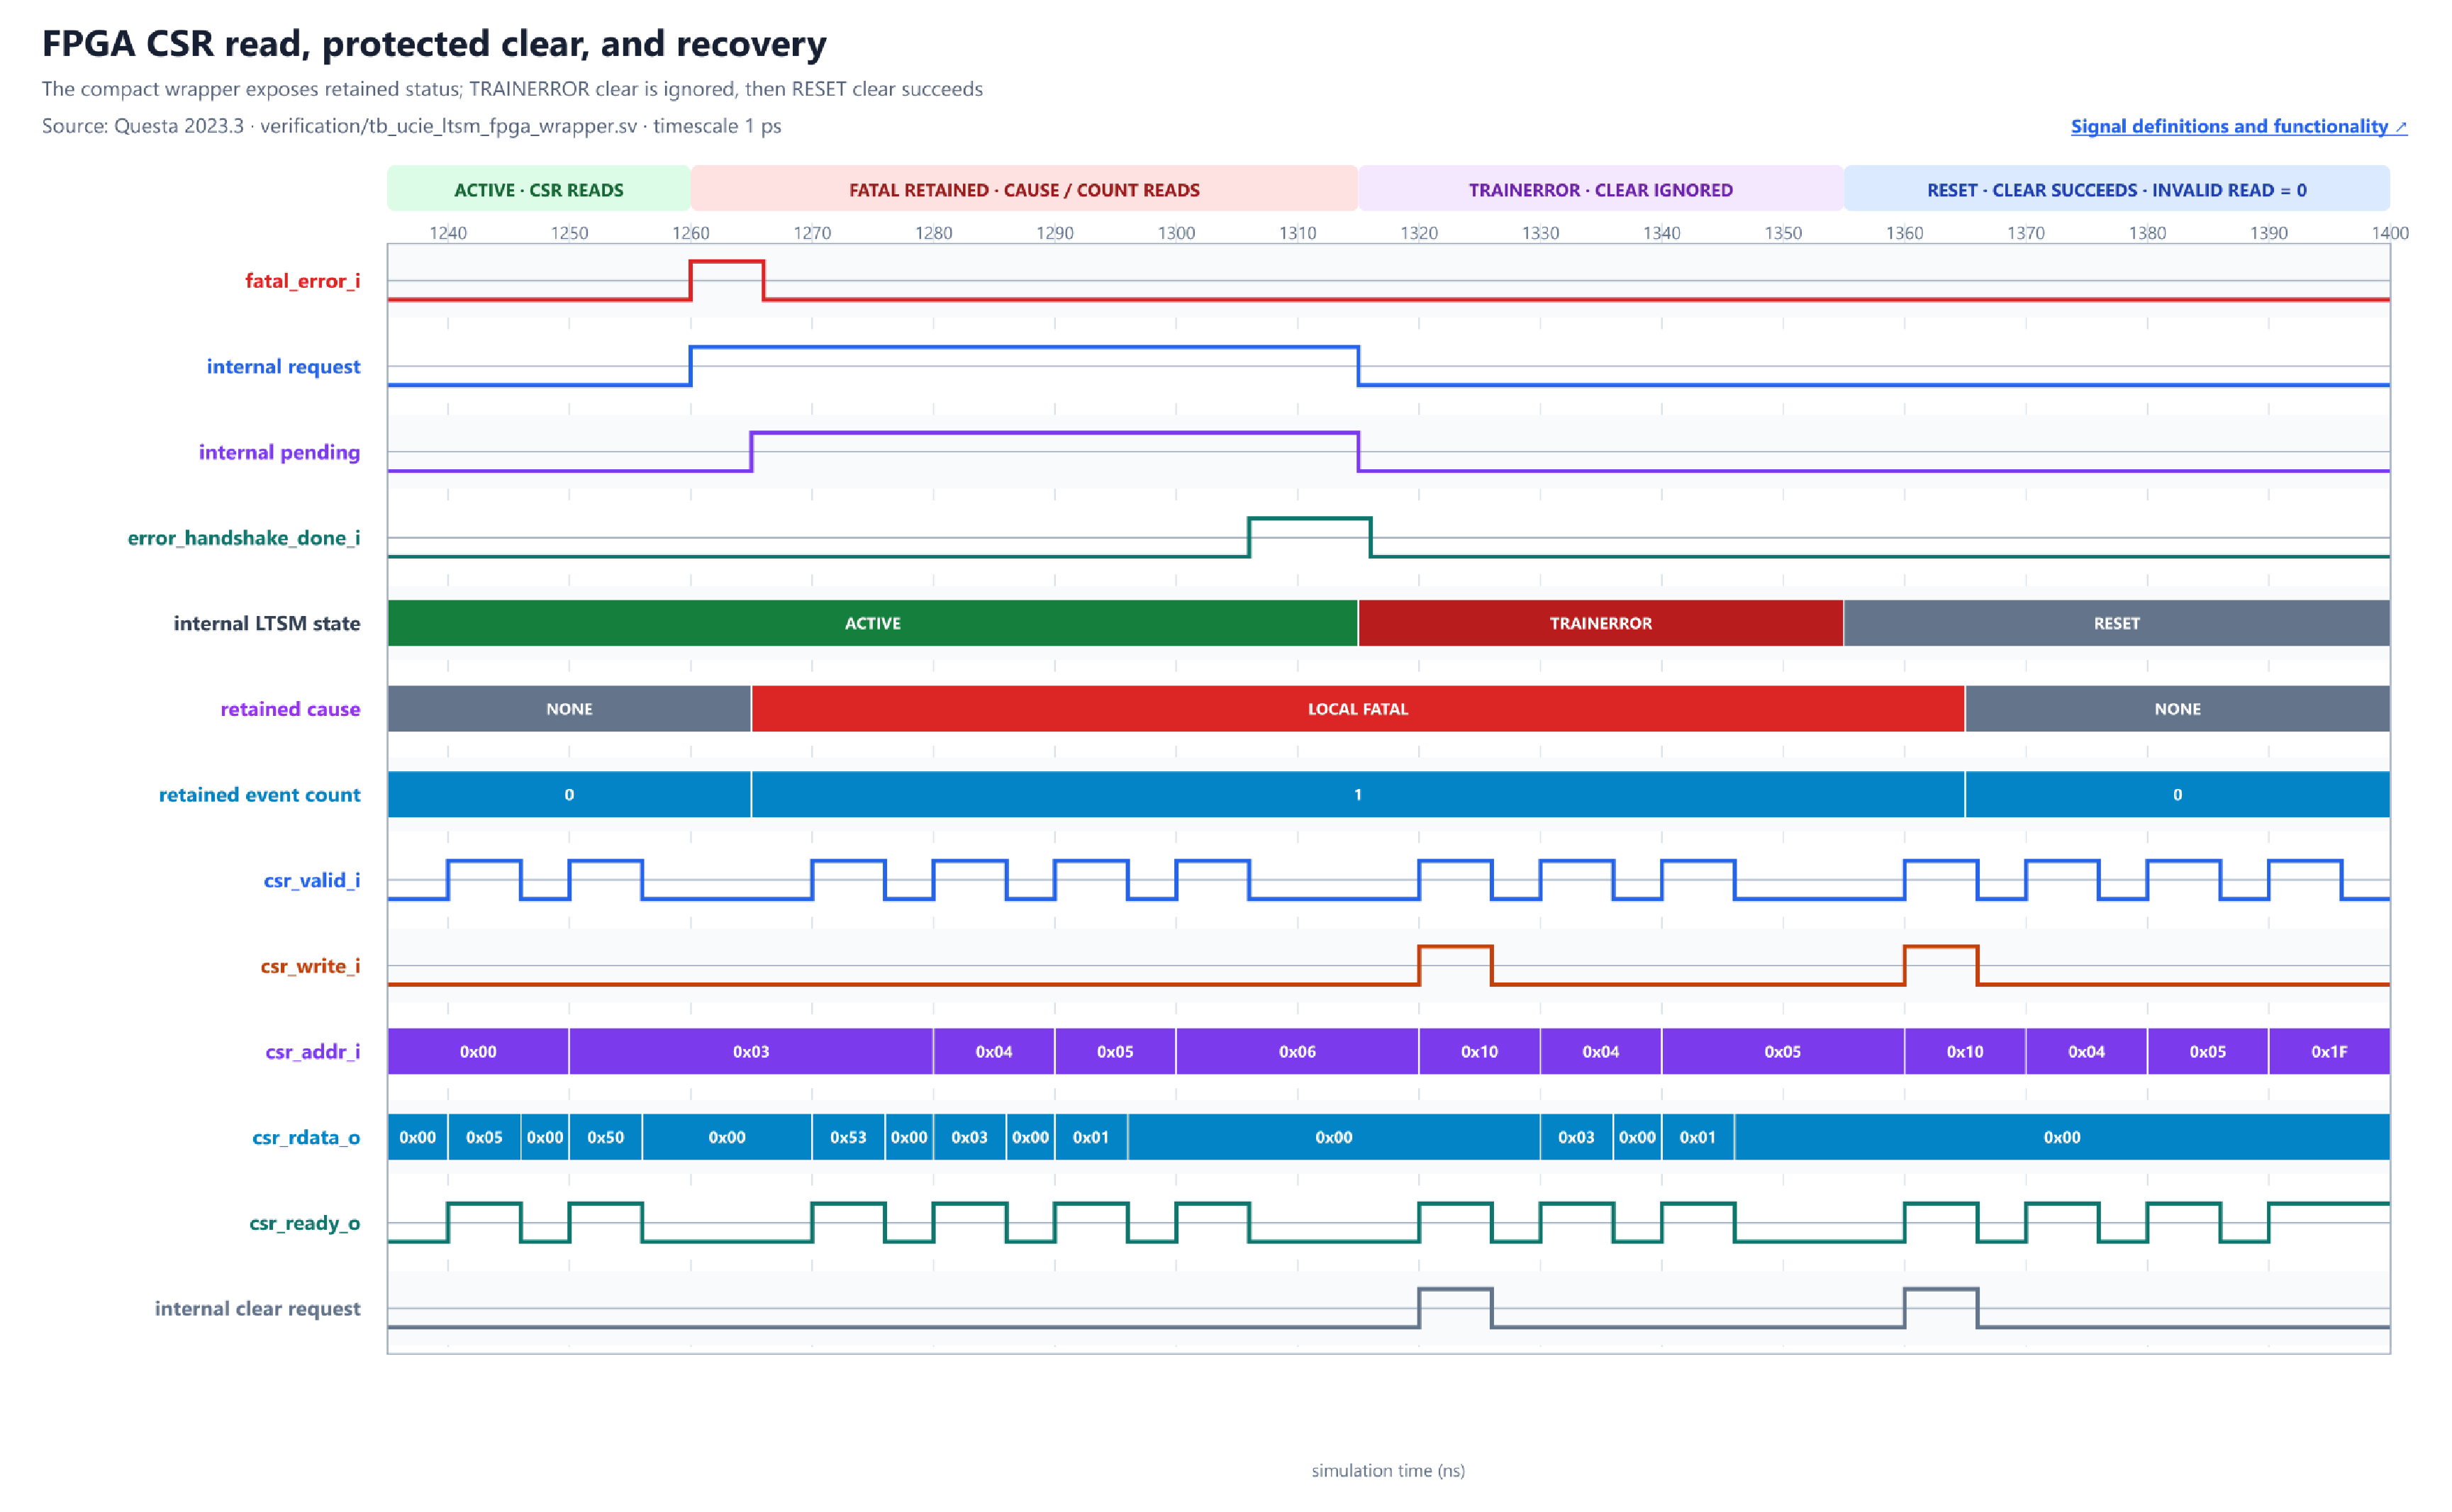
\includegraphics[width=0.97\textwidth]{fig11_wave_csr.pdf}
\caption{Color-coded Questa waveform from the FPGA-wrapper directed test. The
CSR sequence reads retained diagnostics, demonstrates protected and allowed
clear operations, and checks an undefined address.}
\label{fig:wave-csr}
\end{figure*}

\section{Specification-Traceable Verification}
\label{sec:verification}

The verification structure in Fig.~\ref{fig:verification} separates stimulus,
observation, prediction, assertions, and coverage accounting. The separation is
important for training logic: a scoreboard that predicts from the DUT's
internal LFSR state or phase register can agree with the same defect it is meant
to detect.

\begin{figure*}[t]
\centering
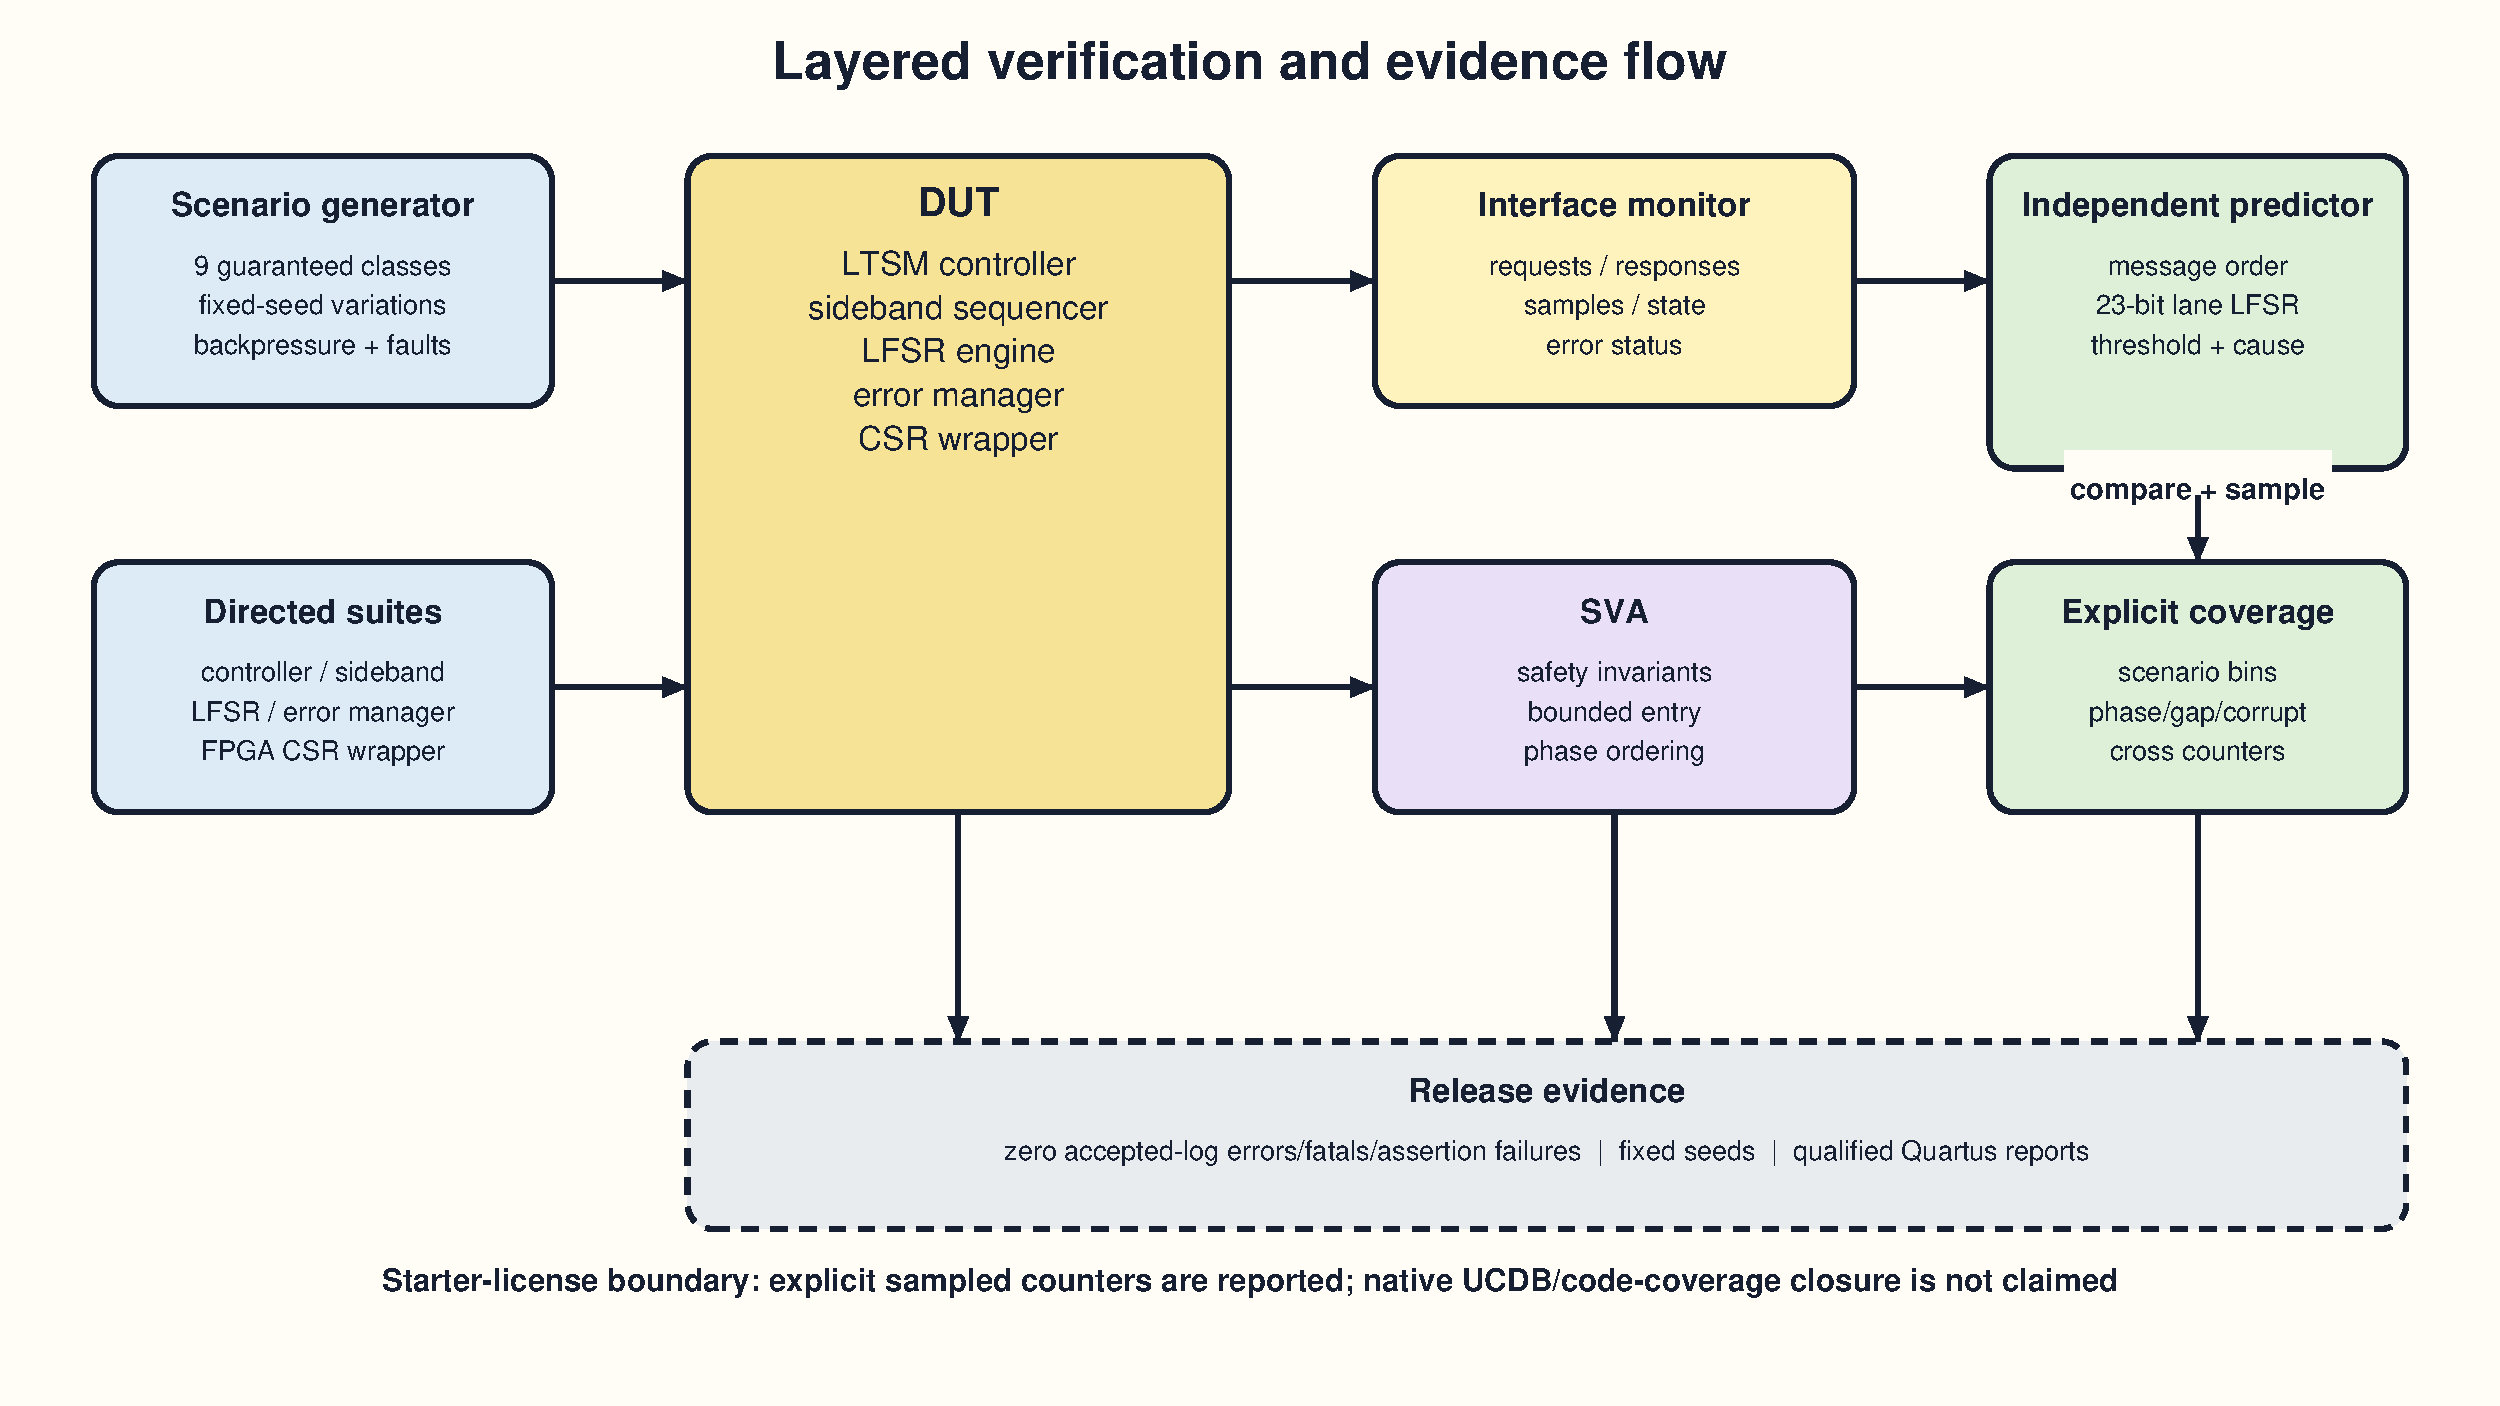
\includegraphics[width=0.86\textwidth]{fig07_verification.pdf}
\caption{Verification architecture. The predictor reconstructs message order,
per-lane LFSR state, thresholds, and error cause from interface observations.}
\label{fig:verification}
\end{figure*}

\subsection{Directed and Randomized Layers}

Directed tests isolate handshake and boundary semantics before integration.
The sideband suite covers successful exchange, timeout/retry, retry exhaustion,
response mismatch, and abort. LFSR tests cover nonzero seeds, the implemented
polynomial, receive gaps, strict threshold equality, abort, the default
4096-sample configuration, and 16-bit saturation. Error-manager tests cover
cause priority, retention, immediate/acknowledged/timed entry, protected clear,
and count saturation. Wrapper tests read version, state, status, training phase,
cause/count, allowed and ignored clear operations, and invalid addresses.

Nine deterministic UVM tests retain top-level state and transition checks.
Separate seeded campaigns stress sideband, training, and recovery behavior.
The production integrated test disables the abstract CENTER1 bypass and uses
nine scenario classes: nominal completion; pattern failure followed by retry
and pass; START retry; malformed START response; END retry; malformed END
response; and reset, fatal, or state-timeout aborts. Backpressure, response
latency, sample gaps, corruption, threshold, and abort phase vary within these
classes.

\subsection{Independent Predictor}

The predictor observes transmitted requests, received responses, accepted
training samples, and public controller/error status. It maintains its own
23-bit state for each of 16 lanes, uses the specified project seed table and
polynomial, advances only when a receive sample is accepted, and computes the
expected mismatch count independently. It also maintains a protocol phase:
START must close before pattern activity, END must not appear before a passing
pattern, and DATATRAINVREF must not be reached until END closes. Abort scenarios
check both clean cessation and retained cause attribution.

\subsection{Assertions and Coverage Boundary}

Concurrent assertions check that \texttt{link\_up} is exclusive to ACTIVE,
timeout routes to TRAINERROR, reset cannot jump directly to ACTIVE, and states
remain known. Integrated assertions restrict pattern activity to
DATATRAINCENTER1/PATTERN, constrain requests to their phase, require an END
response before production-mode advance, check the strict error threshold, and
hold LFSR progress when no sample is accepted. Recovery properties cover
pending request retention, bounded TRAINERROR entry, pending clear, log
stability, and ignored clear in TRAINERROR.

Explicit counters record scenario, phase, gap, corruption, threshold, retry,
abort, and selected cross combinations. They demonstrate that planned classes
were sampled, but are not reported as a standard functional-coverage percentage
because no UCDB was produced under the available Starter license.

\section{Evaluation}
\label{sec:evaluation}

The evaluation asks two bounded questions: whether the production controller
preserves the required START--PATTERN--END ordering under randomized delays and
faults, and whether the same RTL is implementable through a practical FPGA
observability boundary. It does not measure link throughput, latency, BER, or
electrical behavior.

\subsection{Environment and Reproducibility}

Simulation used Questa Intel FPGA Starter Edition 2023.3. The committed
PowerShell and Questa scripts compile the RTL, UVM packages, and assertions,
then run fixed seed lists. The integrated testbench drives a 100-MHz simulation
clock, reduces the training sample count to eight accepted samples, and fixes
\texttt{ALLOW\_ABSTRACT\_DATATRAIN\_BYPASS} to zero. These changes shorten the
experiment without changing the message-order, accepted-sample, threshold, or
abort checks. The RTL default remains 4096 accepted samples.

FPGA mapping, fitting, and timing analysis used Quartus Prime Lite
23.1std.1, targeting a Cyclone 10 LP 10CL025YU256C8G. The SDC applies a
12.5-ns (80-MHz) clock constraint and an asynchronous-reset false path. It does
not assign package locations or external input/output delays; timing values are
therefore internal-clock evidence, not board timing closure.

\subsection{Production Integrated-Training Campaign}

Five seeds each execute 36 trials. Every seed first guarantees all nine
scenario classes and then adds seeded variations in response latency,
backpressure, sample gaps, corruption, threshold, and abort phase. Table
\ref{tab:integrated} reports the accepted per-seed summaries. A request need not
receive a response in malformed-response, retry, or abort cases, and END is
intentionally absent when the pattern does not pass. The resulting count
asymmetry is therefore expected, not packet loss.

\begin{table*}[t]
\caption{Production Integrated-Training Results With Bypass Disabled}
\label{tab:integrated}
\centering
\small
\setlength{\tabcolsep}{4.2pt}
\begin{tabular}{c r rr rr rr rr rrr r}
\toprule
Seed & Trials & \multicolumn{2}{c}{START} & \multicolumn{2}{c}{END} & Retry & Prot. & \multicolumn{2}{c}{Pattern} & \multicolumn{3}{c}{Abort} & Checks \\
 & & Req. & Resp. & Req. & Resp. & & err. & Pass & Fail & Reset & Fatal & T/O & \\
\midrule
1701 & 36 & 36 & 30 & 25 & 17 & 8 & 6  & 25 & 4 & 8 & 1 & 4 & 83 \\
1802 & 36 & 36 & 28 & 23 & 12 & 8 & 11 & 23 & 2 & 3 & 3 & 7 & 76 \\
1903 & 36 & 32 & 28 & 21 & 14 & 5 & 6  & 23 & 4 & 3 & 6 & 7 & 78 \\
2004 & 36 & 34 & 26 & 24 & 18 & 8 & 6  & 23 & 6 & 2 & 3 & 7 & 80 \\
2105 & 36 & 35 & 28 & 27 & 17 & 11& 6  & 27 & 4 & 4 & 5 & 4 & 81 \\
\midrule
Total & 180 & 173 & 140 & 120 & 78 & 40 & 35 & 121 & 20 & 20 & 18 & 29 & 398 \\
\bottomrule
\end{tabular}
\end{table*}

The scenario-hit totals were 18 nominal passes, 20 failed-pattern retry/pass
cases, 17 START retries, 16 malformed START responses, 23 END retries, 19
malformed END responses, 20 reset aborts, 18 fatal aborts, and 29 state-timeout
aborts. Thus all planned classes were observed, while the predictor performed
398 independent order/value/cause checks. The accepted logs report zero UVM
errors and zero UVM fatals, and the regression summary reports no assertion
failures. These observations establish consistency for the committed stimuli;
they are not an exhaustive proof.

\subsection{Preserved Regression Gate}

The integrated campaign was added without discarding earlier evidence. The
release gate also ran nine deterministic UVM tests, 200 sideband trials over
seeds 101--505, 160 LFSR-training trials over seeds 701--1105, and 180 recovery
trials over seeds 1201--1605. Module-directed suites separately exercise the
controller, sideband sequencer, LFSR engine, error manager, and wrapper CSR.
All accepted runs completed without UVM errors/fatals or reported assertion
failures. An ad-hoc ignored debug log is not part of this evidence set.

\subsection{FPGA Mapping, Fit, and Timing}

Table~\ref{tab:fpga} preserves both the positive and negative implementation
results. The wide controller top maps to 763 logic
elements and 505 registers, but demands all 151 device pins; its fitter run
fails. Timing numbers emitted alongside that failed fit are not used as
successful-fit evidence.

The CSR wrapper fits successfully using 824 of 24,624 logic elements (3\%), 505
registers, and 119 of 151 pins (79\%), with no virtual pins. Across the committed
timing corners, the worst setup and hold slacks are +1.013 and +0.179 ns,
respectively, and reported negative slack is zero. The wrapper adds a small
amount of decode logic while reducing external pin demand by 32, demonstrating
why serializing diagnostics is necessary for this device. Because external I/O
constraints and physical pin locations are absent, the result supports
internal synthesizability and fit only \cite{quartusUG}.

\begin{table}[t]
\caption{Cyclone 10 LP Implementation Summary}
\label{tab:fpga}
\centering
\small
\begin{tabular}{lrrr}
\toprule
Metric & Core map & Core fit & Wrapper fit \\
\midrule
Status & success & failure & success \\
Logic elements & 763 & 764 & 824 \\
Registers & 505 & 505 & 505 \\
Pins & 151 & 151 & 119 \\
Setup slack (ns) & -- & -- & +1.013 \\
Hold slack (ns) & -- & -- & +0.179 \\
\bottomrule
\end{tabular}
\end{table}

Fig.~\ref{fig:fpga-evidence} retains the successful and failed implementation
outcomes in one qualified data graphic. Reporting the failed wide-top fit is
important: omitting it would hide the pin-cost reason for the CSR wrapper.

\begin{figure*}[t]
\centering
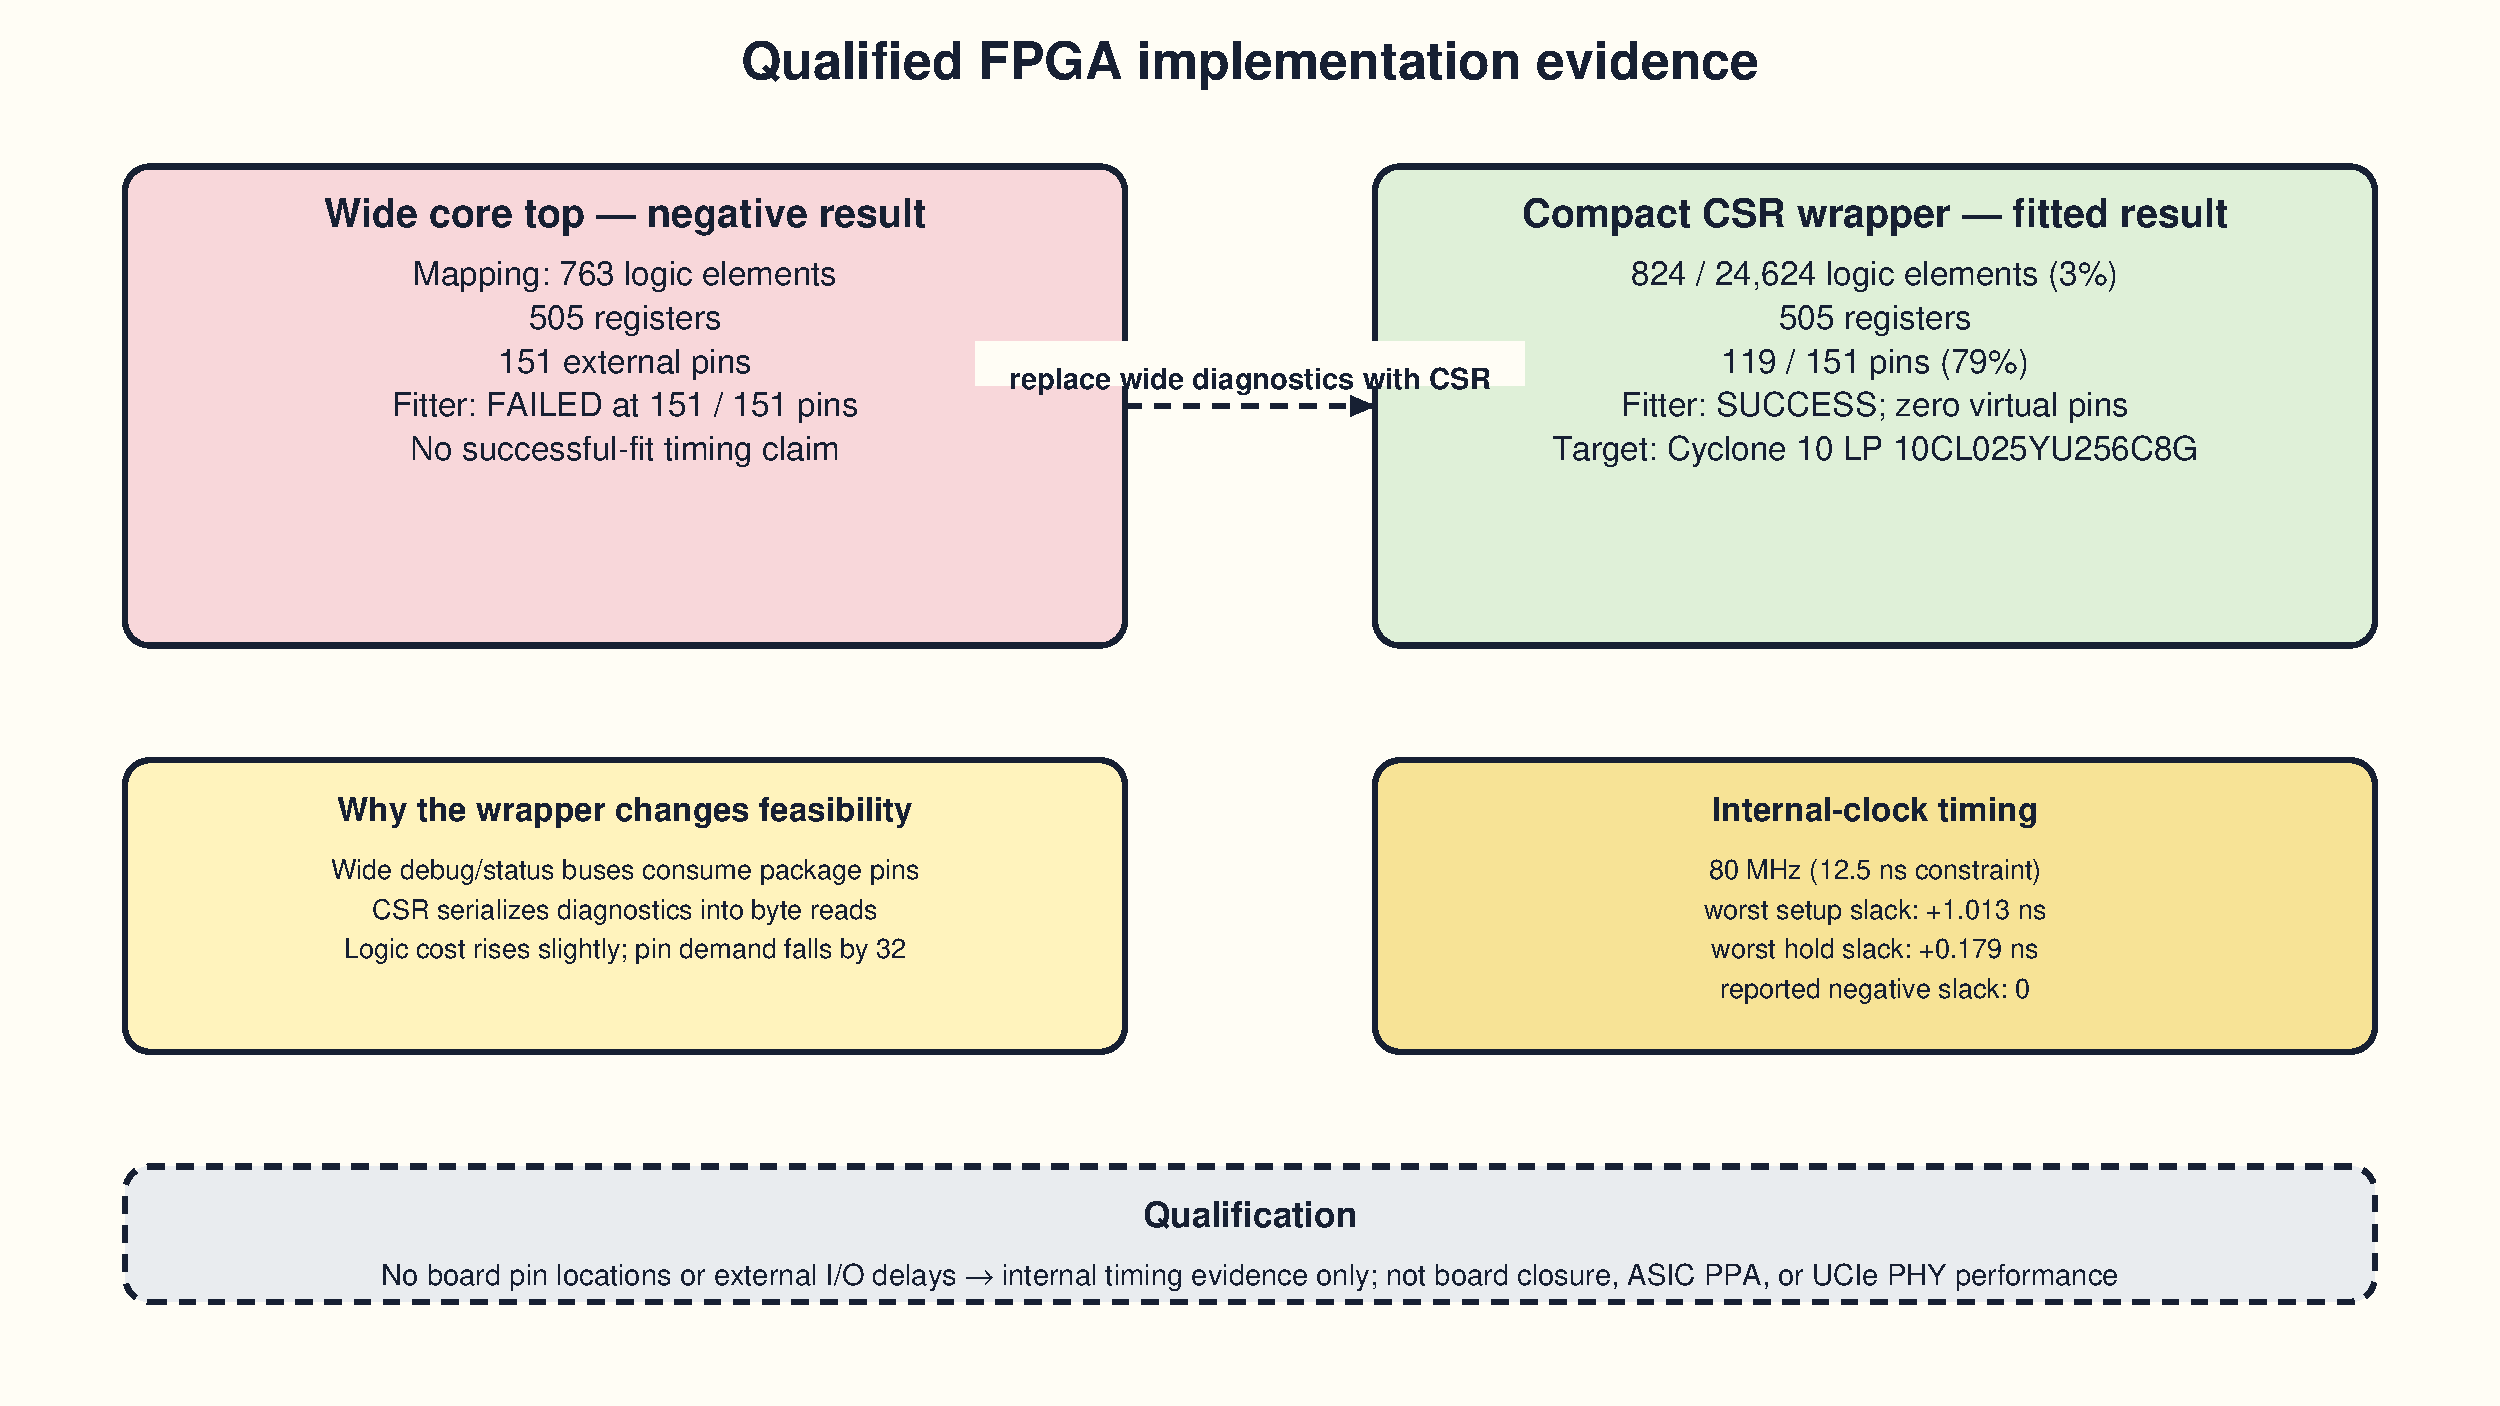
\includegraphics[width=0.92\textwidth]{fig08_fpga_results.pdf}
\caption{Quartus implementation evidence for the same controller under two
observability boundaries. Timing is reported only for the successfully fitted
wrapper and is qualified as internal-clock evidence.}
\label{fig:fpga-evidence}
\end{figure*}

The complete release gate is summarized by Table~\ref{tab:integrated}, the
implementation results in Table~\ref{tab:fpga}, and a
\href{https://github.com/Varadain/ucie-ltsm/blob/feature/v1.0-integrated-training/journal/figures/svg/fig12_regression_evidence.svg}{supplementary release-gate graphic}.
Trial counts are not combined into a coverage percentage because the campaigns
exercise different interfaces and scenario spaces. The supplementary graphic
records which directed, deterministic, randomized, predictor, assertion, and
implementation evidence was preserved together without duplicating those data
as a full-width manuscript float.

\subsection{Threats to Validity}

The pseudo-random campaign uses explicit seeded \texttt{\$urandom\_range}
choices and sampled counters because the Starter license does not support the
native class-randomization and UCDB coverage flow required by the original
plan. No native functional-coverage percentage or code coverage is claimed.
The independent predictor reduces common-mode risk, but design and verification
were developed in the same project. Reduced training counts accelerate
simulation; they do not test full-duration drift. Finally, FPGA synthesis
cannot substitute for a complete two-die model, board experiment, ASIC PPA, or
electrical characterization.

\section{Related Work and Positioning}
\label{sec:related}

Chiplet integration combines smaller dies through advanced packaging to improve
reuse, yield options, and technology specialization, while introducing new
interconnect, test, thermal, and integration challenges
\cite{li2020chiplet,lau2021chiplets}. UCIe addresses the interoperability
problem with a layered die-to-die standard. Sharma \emph{et al.} describe the
architecture, circuit, channel, and packaging rationale behind UCIe 1.0
\cite{sharma2022ucie}; later work examines memory/storage applications
\cite{sharma2024memory} and circuit/package scaling toward three-dimensional
integration \cite{nature2024ucie3d}. Those studies establish UCIe's system and
physical context. This work does not reproduce their bandwidth, energy, or
channel claims; it targets the digital training-control evidence boundary.

Physical UCIe studies further illustrate why that boundary matters. Thermal and
signal-integrity analysis of UCIe-A channels \cite{son2023thermal} and
FPGA-based high-speed interface verification platforms \cite{chang2022fpga}
operate with channel, transceiver, or measurement evidence that is absent here.
Consequently, successful RTL simulation and FPGA fitting cannot imply BER,
electrical margin, or interoperability.

Verification practice commonly combines directed bring-up, constrained-random
exploration, scoreboards, assertions, and coverage. IEEE Std 1800.2 defines the
UVM framework \cite{ieee1800_2}. Vamsikrishna \emph{et al.} describe a unified
testbench supporting directed, random, and pseudo-random operation selection,
including a UCIe-oriented example \cite{vamsi2025unified}. Intel and Cadence
report PHY-model simulation interoperability in which sideband transactions and
high-level LTSM state stepping coordinate vector traffic
\cite{cadenceIntelUcie}. These public accounts demonstrate mature methodology
and commercial model use, but do not provide a directly comparable open RTL
controller, independent lane-LFSR/message-order predictor, retained-error CSR,
and fixed-seed evidence chain.

The contribution here is therefore the auditable combination rather than any
individual technique: a bounded UCIe 2.0-derived RTL control subset, an
interface-derived predictor and SVA layer, explicit negative scenarios, and
qualified FPGA evidence with a preserved failed-fit result. No “first” claim is
made; public literature and proprietary implementations continue to evolve,
including the newer UCIe 3.0 specification \cite{ucie30}.

\section{Discussion}
\label{sec:discussion}

\subsection{What the Evidence Supports}

The strongest result is control-path consistency across independently predicted
message order, per-lane pattern state, threshold decisions, and retained abort
cause. The tests exercise not only nominal completion but also absence
properties: END must not be sent after a failed pattern, DATATRAINVREF must not
be entered before END closes, and illegal clear must not erase a retained
TRAINERROR record. These checks are more informative for the modeled block than
a link-level throughput number that the design cannot produce.

The FPGA result also shows a practical architectural tradeoff. Exposing every
diagnostic directly consumes the complete package-pin budget and fails to fit,
although logic utilization is low. A byte CSR raises logic use from the mapped
763-element core to a fitted 824-element wrapper while reducing pin demand by
32. This is not a performance optimization; it is an observability boundary
that makes the controller implementable on the selected package.

\subsection{What the Evidence Does Not Support}

The controller implements one detailed training operation while delegating most
other substates to \texttt{phase\_done\_i}. The project therefore cannot claim a
complete physical-layer controller. It has no analog front end, package channel,
mainband datapath, protocol adapter, two-die interoperability setup, or official
compliance suite. The Quartus constraint set has no board pin locations or
external I/O delays, and no hardware was measured. There is no ASIC synthesis,
place-and-route, power analysis, CDC/RDC signoff, formal proof, or native code
coverage.

The fixed-seed campaign improves reproducibility but samples a finite behavioral
space. Explicit bin counters confirm that planned classes were exercised; they
do not establish standard coverage closure. A stronger evaluation would run a
licensed native randomization/coverage flow, publish functional and code
coverage with justified exclusions, and use mutation or fault injection to
measure checker sensitivity.

\subsection{Next Experiments}

Three extensions would most improve the scientific claim. First, replace more
phase abstractions with independently checked MBINIT/MBTRAIN procedures and a
two-end behavioral partner. Second, compare controller-only, integrated-engine,
and CSR-wrapper configurations under identical FPGA or ASIC constraints.
Third, add physical credibility through either a fully constrained board build
and hardware experiment or a reproducible ASIC flow with library, PVT,
constraint, area, and power methodology. Until then, the work is best described
as an academic digital-control and verification framework.

\section{Conclusion}

This work develops and audits a UCIe 2.0-derived digital-control subset rather
than a complete link. The RTL joins hierarchical LTSM sequencing, bounded
sideband transactions, per-lane LFSR measurement, retained error attribution,
and a compact FPGA CSR. Production-mode verification keeps the abstract
DATATRAINCENTER1 bypass disabled and uses an independent message-order/LFSR
predictor, assertions, directed corner tests, and fixed-seed negative scenarios.
Across 180 integrated trials, all nine planned scenario classes were observed
with 398 predictor checks and no accepted-log UVM errors or fatals. Earlier
sideband, training, recovery, deterministic, and directed suites also remain in
the regression gate.

On the selected Cyclone 10 LP, the wide diagnostic top fails to fit at 151
pins, while the CSR wrapper fits with 824 logic elements, 505 registers, and
119 pins. Its internal 80-MHz timing reports positive setup and hold slack, but
the absence of board I/O constraints prevents a board-closure claim. The result
is therefore a reproducible academic control/verification artifact. Complete
training procedures, native coverage closure, hardware or ASIC evidence, and
electrical/interoperability validation remain future work.


\section*{Acknowledgment and Tool-Use Disclosure}

The authors must replace this draft text with complete funding, institutional,
conflict-of-interest, and contributor acknowledgments. OpenAI Codex was used
under author direction to assist with repository auditing, evidence
organization, manuscript drafting, and generation of original project figures.
The authors are responsible for independently checking every claim, citation,
figure, result, and disclosure and for approving the final submitted text.

\bibliographystyle{IEEEtran}
\bibliography{references}

% IEEE TVLSI requires biographies for regular papers. Add author photographs
% and IEEEbiography environments only after author metadata is supplied.

\end{document}
